\documentclass{article}

\usepackage[preprint]{neurips_2023}

\usepackage[utf8]{inputenc}
\usepackage[T1]{fontenc}
\usepackage{hyperref}
\usepackage{url}
\usepackage{booktabs}
\usepackage{amsfonts}
\usepackage{amsmath}
\usepackage{nicefrac}
\usepackage{microtype}
\usepackage{xcolor}
\usepackage{graphicx}
\usepackage{multirow}
\usepackage{subcaption}
\usepackage{pifont}

\newcommand{\eva}{EVA-CLIP-18B}
\newcommand{\dino}{DINOv3-7B}
\newcommand{\pp}{\,\mathrm{pp}}

\title{No Free Depth: Exhaustive Layer-Duplication Scans Reveal
Depth-Structured Robustness but No Reasoning Circuits in Large Vision
Transformers}

\author{%
  Amrit Chadha\\
  \texttt{amrit@cerenovus.ai}\\
  \AND
  Claude (Anthropic)\thanks{Experimental infrastructure, analysis tooling,
  and manuscript preparation were carried out with the assistance of Claude
  (Anthropic). All experimental design decisions and claims were reviewed by
  the human author.}\\
}

\begin{document}

\maketitle

\begin{abstract}
Recent work on large language models (LLMs) showed that re-executing a
contiguous block of transformer layers at inference time---without any
weight modification---can \emph{improve} downstream performance, and
attributed this to ``reasoning circuits'' occupying a format-agnostic
middle region of the network. We ask whether this phenomenon transfers to
vision. We exhaustively scan all $L(L{+}1)/2$ contiguous
layer-duplication configurations in the two largest openly available pure
vision transformers spanning both dominant training regimes---\eva{}
(language-supervised, 48 layers, 1{,}176 configurations) and \dino{}
(self-supervised, 40 layers, 820 configurations)---scoring each
configuration with training-free nearest-centroid probes over eleven
datasets that span six real-world domains and five procedurally generated
visual-reasoning tasks. A selection-robust two-stage protocol (borderline
and random test splits, matched noise nulls, per-image bootstrap, and
confirmation of top configurations against random-configuration controls
on held-out images) yields a clear negative: \emph{no} duplication
configuration in either model produces gains that survive confirmation.
The manner of failure, however, is highly structured and informative.
Early-layer duplication is universally destructive; late-layer duplication
is essentially free---the reverse of the LLM finding. A pre-registered
representational-anatomy experiment explains part of this structure: a
content-dominant layer band exists only in the self-supervised model,
where it extends to the final layer, consistent with vision encoders
lacking the ``decode'' phase whose disruption penalizes late-layer
duplication in LLMs. Both models nonetheless exhibit small
($+0.5$--$2\pp$) but statistically reliable second-pass benefits in their
mid-to-late stack. We release all code, per-image outcomes, and analysis
artifacts.
\end{abstract}

\section{Introduction}
\label{sec:intro}

A transformer's forward pass applies a fixed sequence of residual blocks
exactly once. Hankins~\citep{hankins2025rys} demonstrated that this
convention can be profitably violated in large language models: executing
a well-chosen contiguous block of middle layers \emph{twice} at inference
time---reusing the same weights, with no training---improved a 72B-parameter
model's average score across six public benchmarks, with gains up to
$+17.7\pp$ on individual reasoning tasks. Follow-up work generalized the
effect across model families~\citep{hankins2025rysii} and proposed a
mechanism~\citep{hankins2025sapirwhorf}: middle LLM layers operate on a
shared, format-agnostic semantic representation---demonstrated by
cross-lingual similarity analysis---so a middle layer's output is a valid
input to the same region, and a second pass acts as additional
computation in a stable representational space. Early layers (which map
tokens into that space) and late layers (which map it back to token
space) tolerate no such recycling.

Whether any of this transfers to vision is unknown, and the question is
sharper than it may first appear. Vision transformers~\citep{dosovitskiy2021image}
share the residual architecture that makes duplication mechanically
possible, and prior work has found substantial robustness of both CNNs
and LLMs to layer-level perturbation~\citep{huang2016deep,lad2024remarkable}.
But two structural properties differ. First, a vision \emph{encoder}'s
output is already an embedding: there is no analogue of the return to
token space, so the LLM three-phase picture (encode--reason--decode) may
be missing its third phase entirely. Second, the representational content
of a vision model depends on its training objective in a way with no LLM
parallel: a language-supervised model (CLIP-style~\citep{radford2021learning})
is optimized to preserve exactly the appearance attributes---color,
style, background---that a ``format-agnostic content space'' would be
expected to discard, whereas a self-supervised model faces no such
pressure.

We address the question with what is, to our knowledge, the first
exhaustive layer-duplication study in vision, designed around three
methodological commitments:

\begin{enumerate}
\item \textbf{Exhaustiveness and scale.} We scan \emph{every} contiguous
duplication configuration in the largest openly available pure vision
transformer, \eva{}~\citep{sun2024evaclip} (17.5B parameters, 48 layers,
1{,}176 configurations), and repeat the identical experiment on the
largest openly available self-supervised vision transformer,
\dino{}~\citep{simeoni2025dinov3} (40 layers, 820 configurations),
making the training objective the only varied factor.
\item \textbf{Selection-robust inference.} Ranking 1{,}996 configurations
on small probe sets guarantees an inflated maximum (the winner's curse).
Our protocol separates \emph{screening} from \emph{confirmation}: top
configurations are re-evaluated on never-before-used images, with
resampled reference sets, against the empirical distribution of
\emph{random} configurations, under a criterion fixed before the sweep;
complementary controls bound the remaining sources of optimistic bias.
\item \textbf{Registered mechanistic predictions.} Before either sweep
completed, we ran a vision analogue of the cross-lingual anatomy
experiment of \citet{hankins2025sapirwhorf}---an $8{\times}8$
shape-by-rendering-style stimulus grid replacing the original
topic-by-language sentence grid---and recorded the predictions it makes
about each model's duplication tolerance. The sweeps then graded those
predictions.
\end{enumerate}

\textbf{Findings.} The headline result is negative and unambiguous: in
neither training regime does any duplication configuration produce
improvements that survive selection-robust confirmation. RYS-style free
gains do not transfer to vision-transformer representation quality at the
scales tested. The structure of the negative result is the paper's
positive contribution:

\begin{itemize}
\item \textbf{Depth-structured tolerance, inverted relative to LLMs.}
Early-layer duplication is destructive in every dataset and both models;
mid-stack duplication is nearly free; late-stack duplication is
essentially undetectable ($|\Delta|<0.4\pp$)---whereas in LLMs
late-layer duplication is catastrophic.
\item \textbf{The content band is an objective effect, not an
architecture effect.} The anatomy experiment finds \emph{no}
content-dominant layer band anywhere in \eva{}: rendering style dominates
its representational geometry at all 48 layers. In \dino{} a
content-dominant band exists (layers 35--40 under CLS pooling; 28--40
under patch pooling)---and it extends to the \emph{final} layer,
consistent with the missing-decode-phase account of late-layer immunity.
\item \textbf{Small but real second-pass effects.} Top configurations in
both models reproduce small positive deltas on held-out images with
bootstrap confidence intervals excluding zero ($+1.2$ to $+2.0\pp$ in
\eva{}'s late-middle stack; $+0.5$ to $+0.8\pp$ in \dino{}'s mid-stack),
yet remain within what arbitrary-configuration luck can produce under the
pre-specified control-band test.
\item \textbf{A quantitative robustness gap between training regimes.}
Averaged over all configurations and datasets, duplication costs \eva{}
$-5.8\pp$ but \dino{} only $-0.7\pp$: the self-supervised model is
roughly an order of magnitude more tolerant of depth recycling.
\end{itemize}

All code, figures, per-image outcomes, and the complete decision log are
available at \url{https://github.com/avchadha/rys}.

\section{Background and Related Work}
\label{sec:related}

\textbf{Layer duplication in LLMs.} \citet{hankins2025rys} introduced the
configuration space studied here: for a network with layers
$0,\dots,L{-}1$, a configuration $(i,j)$ executes layers
$0..j{-}1$, feeds the hidden state after layer $j{-}1$ back into layer
$i$, re-executes layers $i..j{-}1$, and continues with layers $j..L{-}1$.
On Qwen2-72B, the optimal seven-layer block $(45,52)$ raised the Open LLM
Leaderboard average by $+2.61\pp$. \citet{hankins2025rysii} replicated
the phenomenon across families, introduced single-layer $k$-fold
repetition, and framed results as a quality/compute Pareto frontier;
\citet{hankins2025sapirwhorf} provided the representational account.

\textbf{Depth recycling and adaptive depth.} Re-executing layers is the
inference-time limit of a family of ideas that treat transformer depth as
a flexible resource. Universal Transformers tie weights across
depth---every layer is, by construction, a repetition of one
block---and gain algorithmic generalization from
recurrence~\citep{dehghani2019universal}; recurrent ``deep-thinking''
networks extrapolate to harder problem instances simply by iterating a
learned block longer~\citep{schwarzschild2021can}. Both findings supply
the prior that made RYS plausible: extra passes through the right
computation can help. On the deployment side, depth
up-scaling~\citep{kim2024solar} physically duplicates layer blocks and
then fine-tunes; CALM exits language models early when
confident~\citep{schuster2022confident}; LayerSkip trains for early exit
and reuses skipped depth for self-speculative
decoding~\citep{elhoushi2024layerskip,zhang2024draft}; Mixture-of-Depths
routes tokens past layers dynamically~\citep{raposo2024mixture}. Vision
has analogous early-exit and adaptive-token
architectures~\citep{huang2018multi,yin2022avit}, but all such designs
\emph{train for} depth flexibility. What has been missing---and what this
paper contributes---is a map of how much depth flexibility large vision
transformers possess \emph{without any training}, measured exhaustively rather than at
designer-chosen exit points; duplication is the mirror image of the layer
\emph{deletion} studied by~\citet{lad2024remarkable}, probing the same
question of where the residual stream tolerates a depth--computation
mismatch.

\textbf{Layer-level robustness and interpretability.} Networks tolerate
substantial layer-level perturbation: stochastic depth trains CNNs with
randomly dropped layers~\citep{huang2016deep}; LayerDrop does the same
for transformers~\citep{fan2020reducing}; \citet{lad2024remarkable}
find LLMs robust to deleting or swapping adjacent middle layers, and
propose a stages-of-inference picture consistent with the anatomy used
here. Intermediate-representation probing goes back at least to linear
classifier probes~\citep{alain2017understanding} and the logit
lens~\citep{nostalgebraist2020logitlens}; the cross-lingual variant we
adapt~\citep{hankins2025sapirwhorf} is closely related to findings that
multilingual LLMs route computation through a shared latent
space~\citep{wendler2024llamas}. In vision, \citet{raghu2021vision}
characterize depth-wise representation structure in ViTs; our anatomy
experiment adds a content/style factorization to that program.

\textbf{Models.} \eva{}~\citep{sun2024evaclip} is, to our knowledge, the
largest openly released pure vision transformer (17.5B-parameter vision
tower; contrastive language supervision). \dino{}~\citep{simeoni2025dinov3}
is the largest openly released self-supervised vision transformer
(6.7B parameters, image-only distillation with Gram anchoring). Google's
ViT-22B~\citep{dehghani2023scaling} is larger but not publicly released.
Vision-language assistants were excluded deliberately: their vision
towers are small (e.g., Qwen2.5-VL couples a $\sim$0.7B ViT to LLMs up to
72B), and measuring duplication through a downstream LLM confounds the
representational effect with the LLM's tolerance to perturbed inputs
(Appendix~\ref{app:excluded}).

\section{Method}
\label{sec:method}

\subsection{The duplication operator and exhaustive scan}
\label{sec:operator}

Let $h_k$ denote the hidden state after block $k$ of an $L$-block
encoder. Configuration $(i,j)$, $0 \le i < j \le L$, computes the
standard forward pass to $h_{j-1}$,\footnote{Throughout, block indices
are zero-based; $j$ is exclusive, so $(i,j)$ duplicates the $j{-}i$
blocks $i,\dots,j{-}1$.} re-enters block $i$ with $h_{j-1}$ as input,
re-executes blocks $i..j{-}1$, and continues normally. No weights,
normalization statistics, or position information are modified. We scan
\emph{all} $L(L{+}1)/2$ configurations (1{,}176 for \eva{}; 820 for
\dino{}), avoiding any grid or sampling artifacts: any contiguous
structure observed in the resulting maps is real. A cached implementation
makes this tractable: one baseline pass per image batch caches all $L{+}1$
intermediate states, after which configuration $(i,j)$ costs only
$(j{-}i) + (L{-}j)$ block evaluations. Equality of the cached and direct
paths is verified in unit tests and against each real checkpoint before
any scan. We additionally scan single-layer $k$-fold repetitions
($k \in \{3,4\}$, exploratory; \S\ref{sec:krepeat}).

Features are read from each model's \emph{trained output interface}: the
post-layer-norm CLS token for \eva{}, and the final-norm CLS token for
\dino{}---applied identically to baseline and duplicated passes, so
deltas are attributable solely to the intervention.
Table~\ref{tab:scale} summarizes the scale of the resulting experiment.

\begin{table}[t]
\caption{\textbf{Scale of the experiment.} Sweep evaluations =
configurations $\times$ datasets; every evaluation scores two test splits
and two metrics, with per-image outcomes persisted. Confirmation
re-scores 40 configurations per model (top-20 + 20 random controls) on
500 fresh images per dataset.}
\label{tab:scale}
\centering
\small
\begin{tabular}{lcccccc}
\toprule
Model & Params & $L$ & Configs & Sweep evals & $k$-repeat evals & GPU-h \\
\midrule
\eva{}~\citep{sun2024evaclip} & 17.5B & 48 & 1{,}176 & 12{,}936 & 1{,}056 & 27.5 \\
\dino{}~\citep{simeoni2025dinov3} & 6.7B & 40 & 820 & 9{,}020 & 880 & 6.0 \\
\midrule
Total & & & 1{,}996 & 21{,}956 & 1{,}936 & 33.5 \\
\bottomrule
\end{tabular}
\end{table}

\subsection{Task battery}
\label{sec:tasks}

Following the logic of the original study---whose probes (mathematics and
emotional inference) were chosen to engage \emph{different} putative
circuits---we evaluate eleven datasets spanning distinct visual domains
and distinct visual computations. Six are real-world:
ImageNet~\citep{deng2009imagenet} (100-class subset), DTD
textures~\citep{cimpoi2014describing}, EuroSAT satellite
imagery~\citep{helber2019eurosat}, Places365
scenes~\citep{zhou2018places} (100-class subset), Stanford~40
actions~\citep{yao2011human}, and FGVC-Aircraft~\citep{maji2013fine}.
Five are procedurally generated visual-reasoning probes, each isolating
one computation with explicit confound controls (Appendix~\ref{app:synthetic}):
\emph{counting} (numerosity, 10 classes; non-overlapping dots with
count-independent radius distributions), \emph{same/different}
(relational identity; area-matched distractors), \emph{spatial relation}
(4-way relative position; jittered reference), \emph{symmetry} (mirror
detection; matched per-half color/size/position marginals), and
\emph{inside/outside} (topology; boundary-margin and annulus
constraints).

\subsection{Probing and debiased evaluation}
\label{sec:probes}

Each configuration is scored by \emph{training-free} nearest-centroid
classification with cosine similarity: class centroids are means of
reference-image embeddings, recomputed \emph{within each configuration's
feature space}. Unlike a trained probe, this readout cannot adapt to (and
thereby mask) representation degradation~\citep{alain2017understanding}.
Reference budgets scale inversely with class count
($n_{\mathrm{ref}}/\mathrm{class} = \mathrm{clip}(\lceil 150/C \rceil, 5, 50)$),
equalizing centroid reliability across datasets.

\textbf{Two test splits.} A pilot analysis showed that the natural
choice---testing on the images the baseline model finds
\emph{hardest}---guarantees spurious positive deltas: with baseline
accuracy pinned near zero on an adversarially selected set, \emph{any}
perturbation, including pure noise, regresses toward the mean. We instead
draw, per dataset, (i) a \emph{borderline} split of 100 images stratified
around the decision boundary (50 barely misclassified, 50 barely correct,
by $|$cosine margin$|$), on which baseline accuracy is $\approx 50\%$ by
construction and deltas can move in both directions; and (ii) a
\emph{random} control split of 100 images, disjoint from the borderline
split, whose deltas are unbiased. \textbf{All rankings and headline
statistics use the random split}; the borderline split is reported to
quantify selection sensitivity (Appendix~\ref{app:selection}).

\textbf{Noise null.} For each dataset we measure the $\Delta$accuracy
distribution produced by adding isotropic Gaussian noise of relative
magnitude $\alpha \in \{0.005,\dots,0.1\}$ to both reference and test
features (20 seeds each). This weak lower-bound null never exceeded
$+0.9\pp$ on the random split for \eva{} ($+2.5\pp$ for \dino{}'s
near-ceiling same/different), confirming that the debiased splits do not
manufacture positive effects.

\textbf{Uncertainty.} Per-image correctness and true-class rank are
persisted for every (configuration, dataset, split); confidence intervals
are paired bootstrap over images within dataset (2{,}000 resamples,
datasets treated as fixed effects), with configuration and baseline
evaluated on identical resamples.

\subsection{Two-stage selection-robust confirmation}
\label{sec:confirm}

With $\sim$1{,}000 configurations evaluated on 100-image splits
(per-cell standard error $\approx 3$--$5\pp$), the expected maximum under
the global null is $+15$--$20\pp$: sweep-stage leaders are inflated by
construction. Stage two therefore re-evaluates the top 20 configurations
(ranked by $z$-scored random-split aggregate; Appendix~\ref{app:agg})
\emph{plus 20 random control configurations} on 500 fresh test images per
dataset (disjoint from the entire stage-one candidate pool) with
resampled reference sets. The pre-specified confirmation criterion,
fixed before either sweep ran, is
\begin{equation}
\label{eq:criterion}
\mathrm{CI}_{95}(\Delta) > 0 \quad \wedge \quad
\Delta > \mu_{\mathrm{ctrl}} + 2\sigma_{\mathrm{ctrl}},
\end{equation}
i.e., a configuration must beat both zero and the empirical distribution
of arbitrary duplications evaluated under identical conditions. This is
the analogue of \citet{hankins2025rysii}'s ``small probes guide search;
large probes judge candidates.''

\subsection{Representational anatomy with registered predictions}
\label{sec:anatomy}

\citet{hankins2025sapirwhorf} measured, at every layer of an LLM,
centered pairwise cosine similarities over an $8{\times}8$
topic-by-language sentence grid, finding a middle region where
same-topic/different-language pairs are more similar than
same-language/different-topic pairs---a content-dominant band that
coincides with duplication tolerance. Our vision translation replaces
language with \emph{rendering style} and topic with \emph{shape
identity}: eight shape classes rendered in eight styles (solid, outline,
inverted, stippled, striped, sketch, on-black, cluttered background), two
jittered instances per cell (128 images; Appendix~\ref{app:grid}).
At every layer we pool token representations (CLS primary; patch-mean
secondary\footnote{The style axis mostly manipulates backgrounds, which
dominate a patch-mean over $\sim$75\% of the canvas; CLS is both the
model's own learned summary and the exact vector used by the duplication
probes. Patch pooling excludes each model's prefix tokens (one CLS for
\eva{}; CLS plus four registers~\citep{darcet2024vision} for \dino{}).}),
center pairwise cosine similarities per layer, and average within pair
categories. The \emph{content band} is the set of layers where the
same-content curve exceeds the same-style curve.

Critically, the anatomy runs \emph{before} each model's sweep completes,
and its predictions were recorded in the project's methods log with
timestamps: for \eva{} (no band found), \emph{duplication should be
broadly harmful with no beneficial band}; for \dino{} (band at layers
28--40), \emph{tolerance and any gains should concentrate in that band,
with early layers fragile}. Section~\ref{sec:scorecard} grades both.

\section{Results}
\label{sec:results}

\subsection{Anatomy: the content band is a training-objective effect}
\label{sec:anatomyresults}

\begin{figure}[t]
\centering
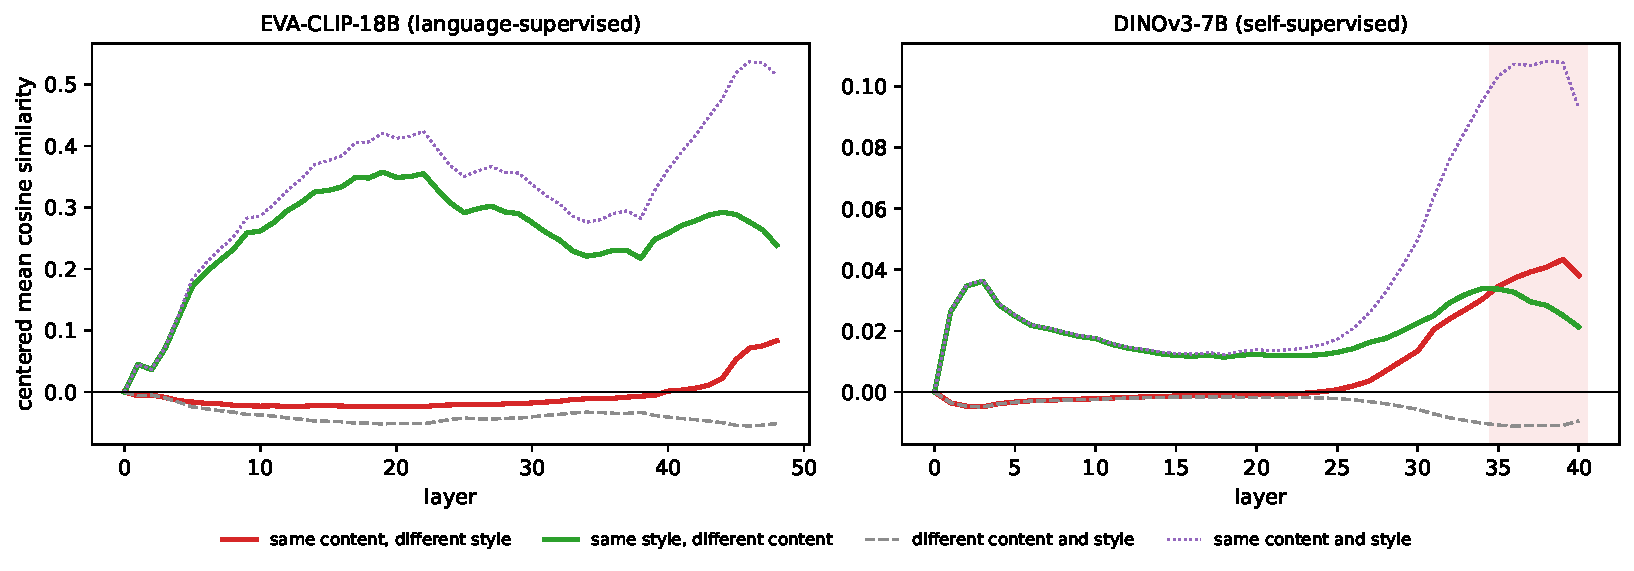
\includegraphics[width=\linewidth]{figures/anatomy_comparison.pdf}
\caption{\textbf{Layer anatomy under CLS pooling} for the
language-supervised (left) and self-supervised (right) model. Curves show
per-layer-centered mean pairwise cosine similarity for pairs sharing
content (shape) but not style, style but not content, neither, or both
(ceiling). In \eva{}, style organization dominates at \emph{every} layer
(final-layer content-minus-style gap $-0.155$). In \dino{}, content
overtakes style in a band (shaded) covering layers 35--40---extending to
the network's final layer, unlike the LLM case where the band closes
$\sim$15 layers before the output.}
\label{fig:anatomy}
\end{figure}

Figure~\ref{fig:anatomy} shows the central mechanistic result. In \eva{},
the same-style curve exceeds the same-content curve at all 48 layers: at
no depth does the model's representational geometry organize the stimulus
grid primarily by shape identity. The content-minus-style gap is
maximally $0.000$ (at the input embedding, where the CLS token is
input-independent) and $-0.155$ at the final layer. Under patch-mean
pooling the gap rises monotonically with depth from $-0.69$
(background-dominated) to $-0.03$ at layer 45 without ever crossing zero.
In \dino{}, by contrast, the content curve overtakes style at layer 35
and remains dominant through the final layer 40 (CLS pooling; maximum gap
$+0.018$; final-layer gap $+0.017$); patch pooling widens the band to
layers 28--40.

Two conclusions follow. First, \emph{the absence of a content band in
\eva{} is attributable to language supervision, not to vision-transformer
architecture}: stimuli and analysis are held fixed between the models.
For a caption-matching objective, rendering style and background
\emph{are} content---a caption of a white star on purple mentions the
purple---echoing, in representational geometry, known appearance biases
of contrastively trained models~\citep{geirhos2019imagenet}. Second, \dino{}'s band runs to
the final layer. In LLMs the content band closes well before the output
because the network must re-enter token space~\citep{hankins2025sapirwhorf};
an encoder whose output \emph{is} the embedding has nowhere to return to.
This is the registered no-decode-phase signature, and it predicts the
late-layer duplication immunity observed next. We note the gap magnitudes
($\sim$0.02) are far smaller than their LLM counterparts: style remains
strongly represented even in \dino{}.

\subsection{Exhaustive sweeps: depth-structured tolerance, inverted
relative to LLMs}
\label{sec:sweeps}

\begin{figure}[t]
\centering
\begin{subfigure}[t]{0.495\linewidth}
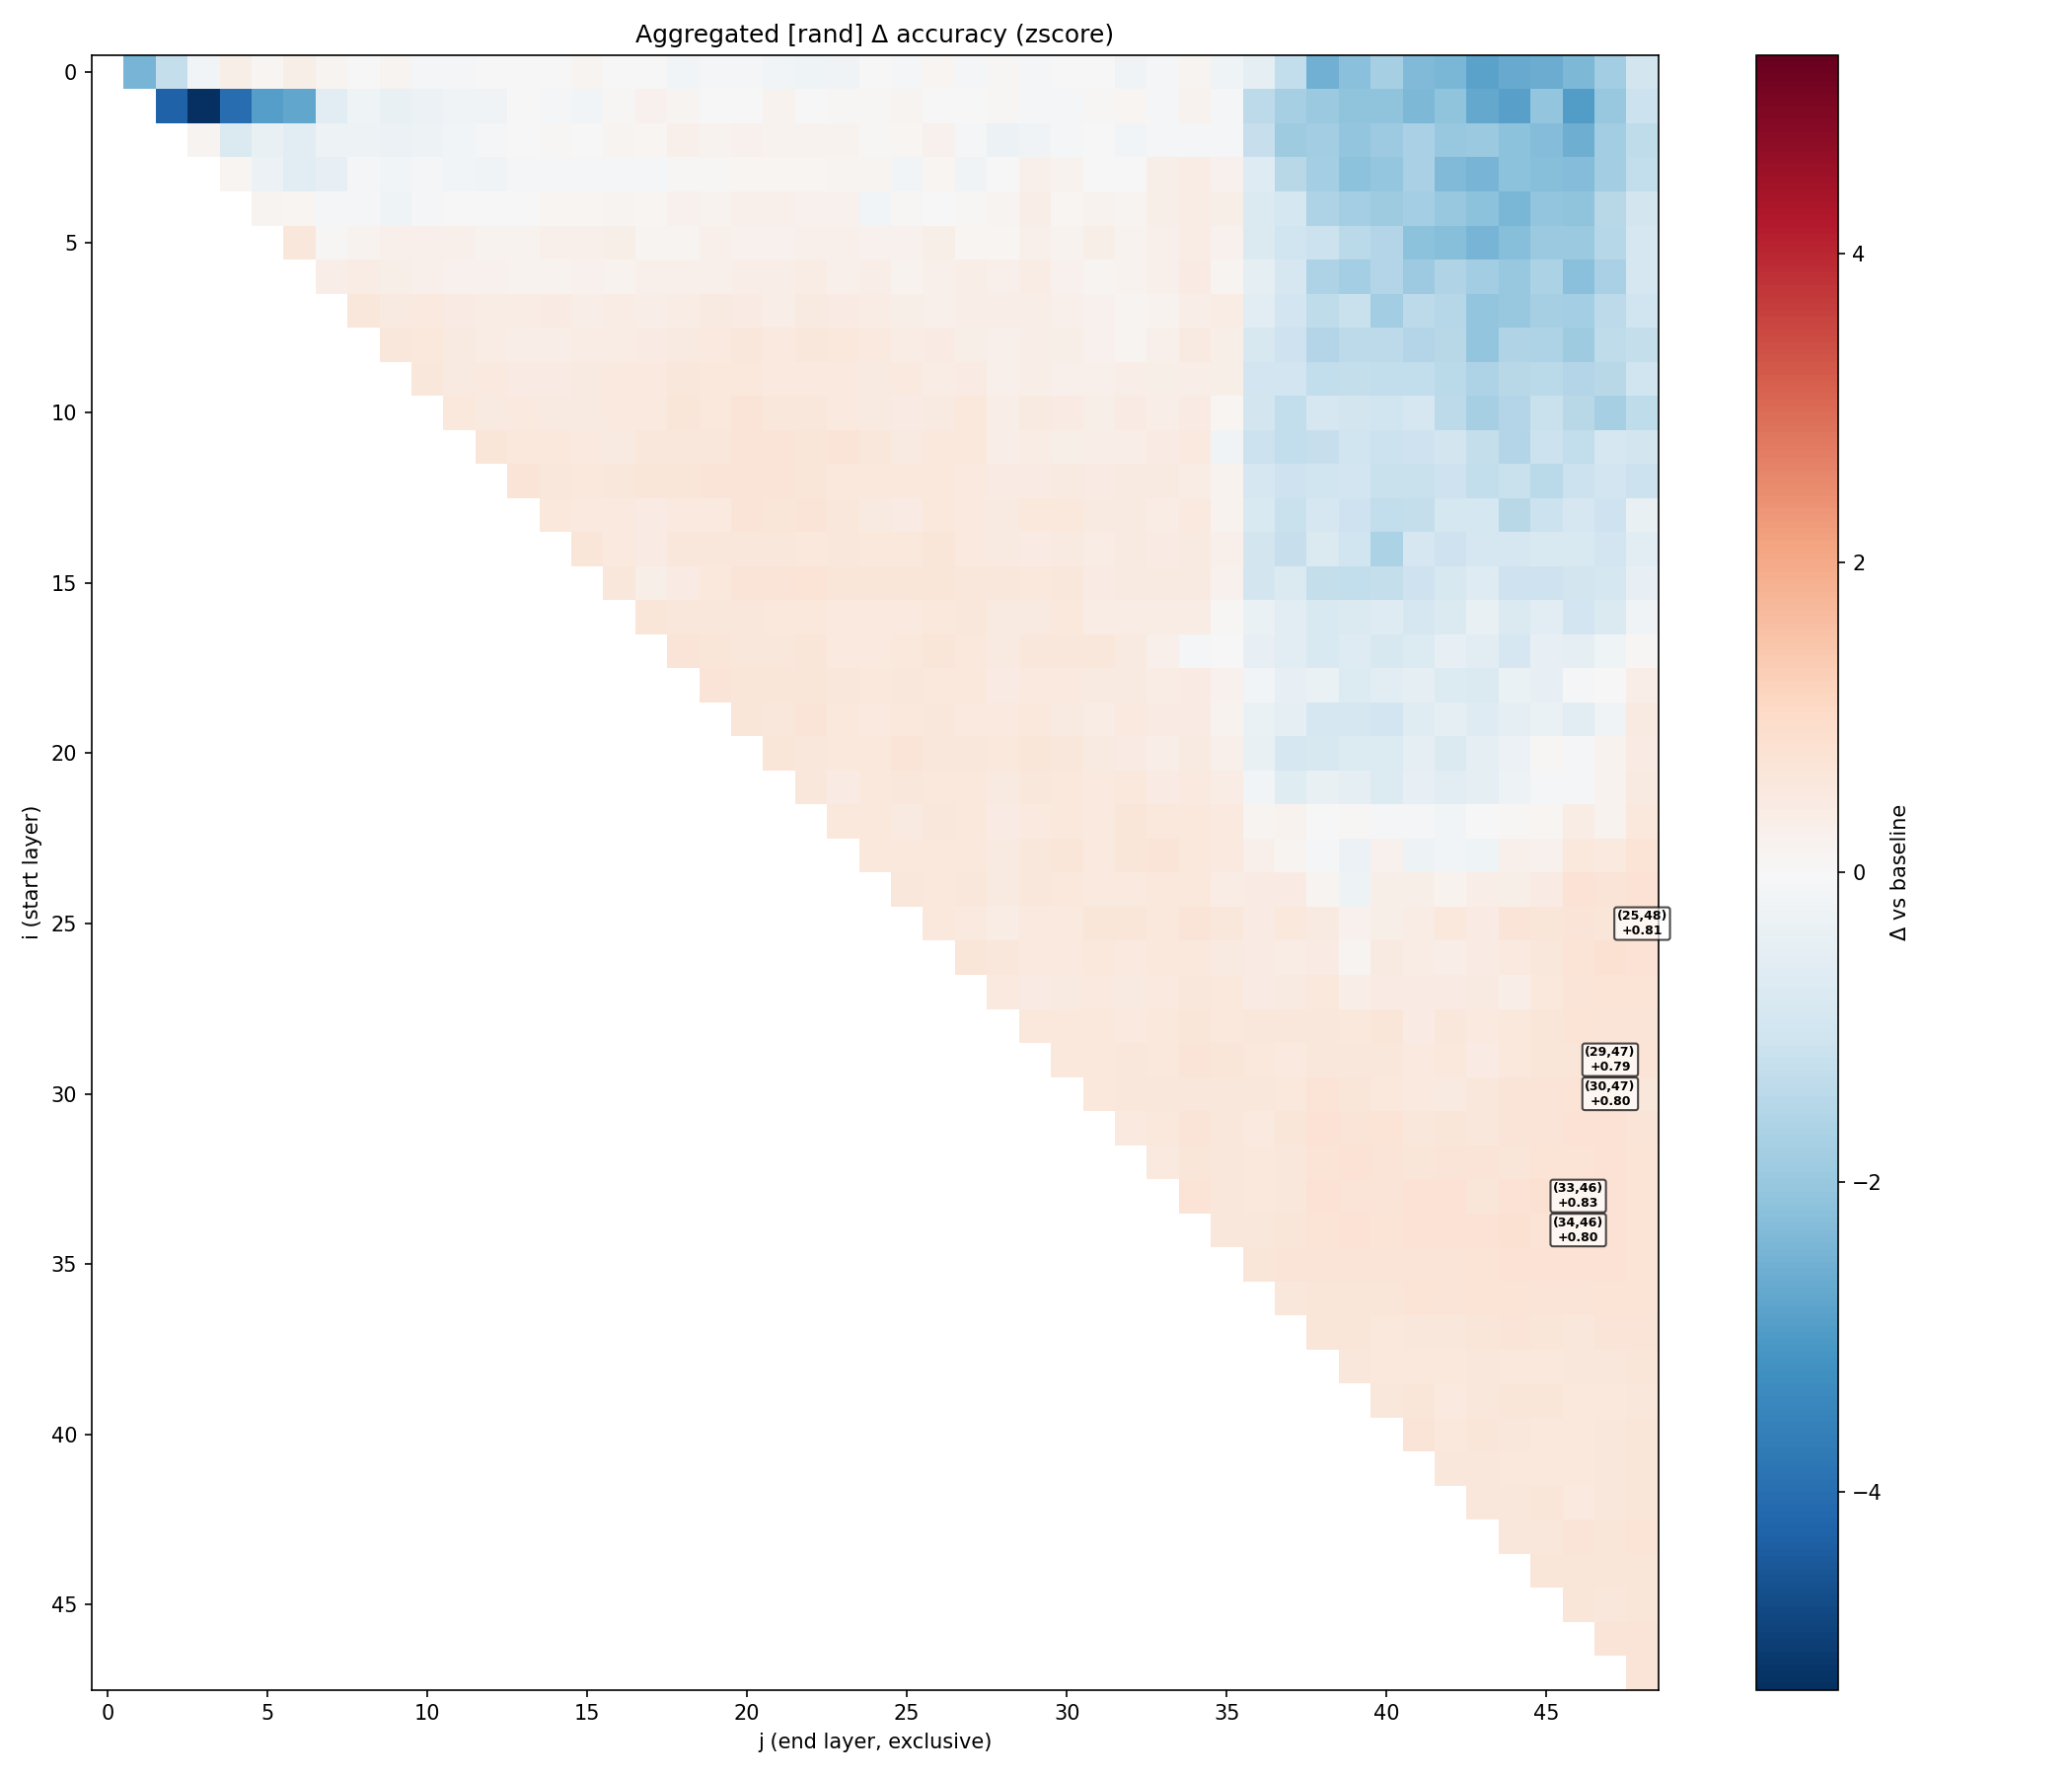
\includegraphics[width=\linewidth]{figures/eva_agg_zscore.png}
\caption{\eva{} (48 layers, 1{,}176 configurations)}
\end{subfigure}
\hfill
\begin{subfigure}[t]{0.495\linewidth}
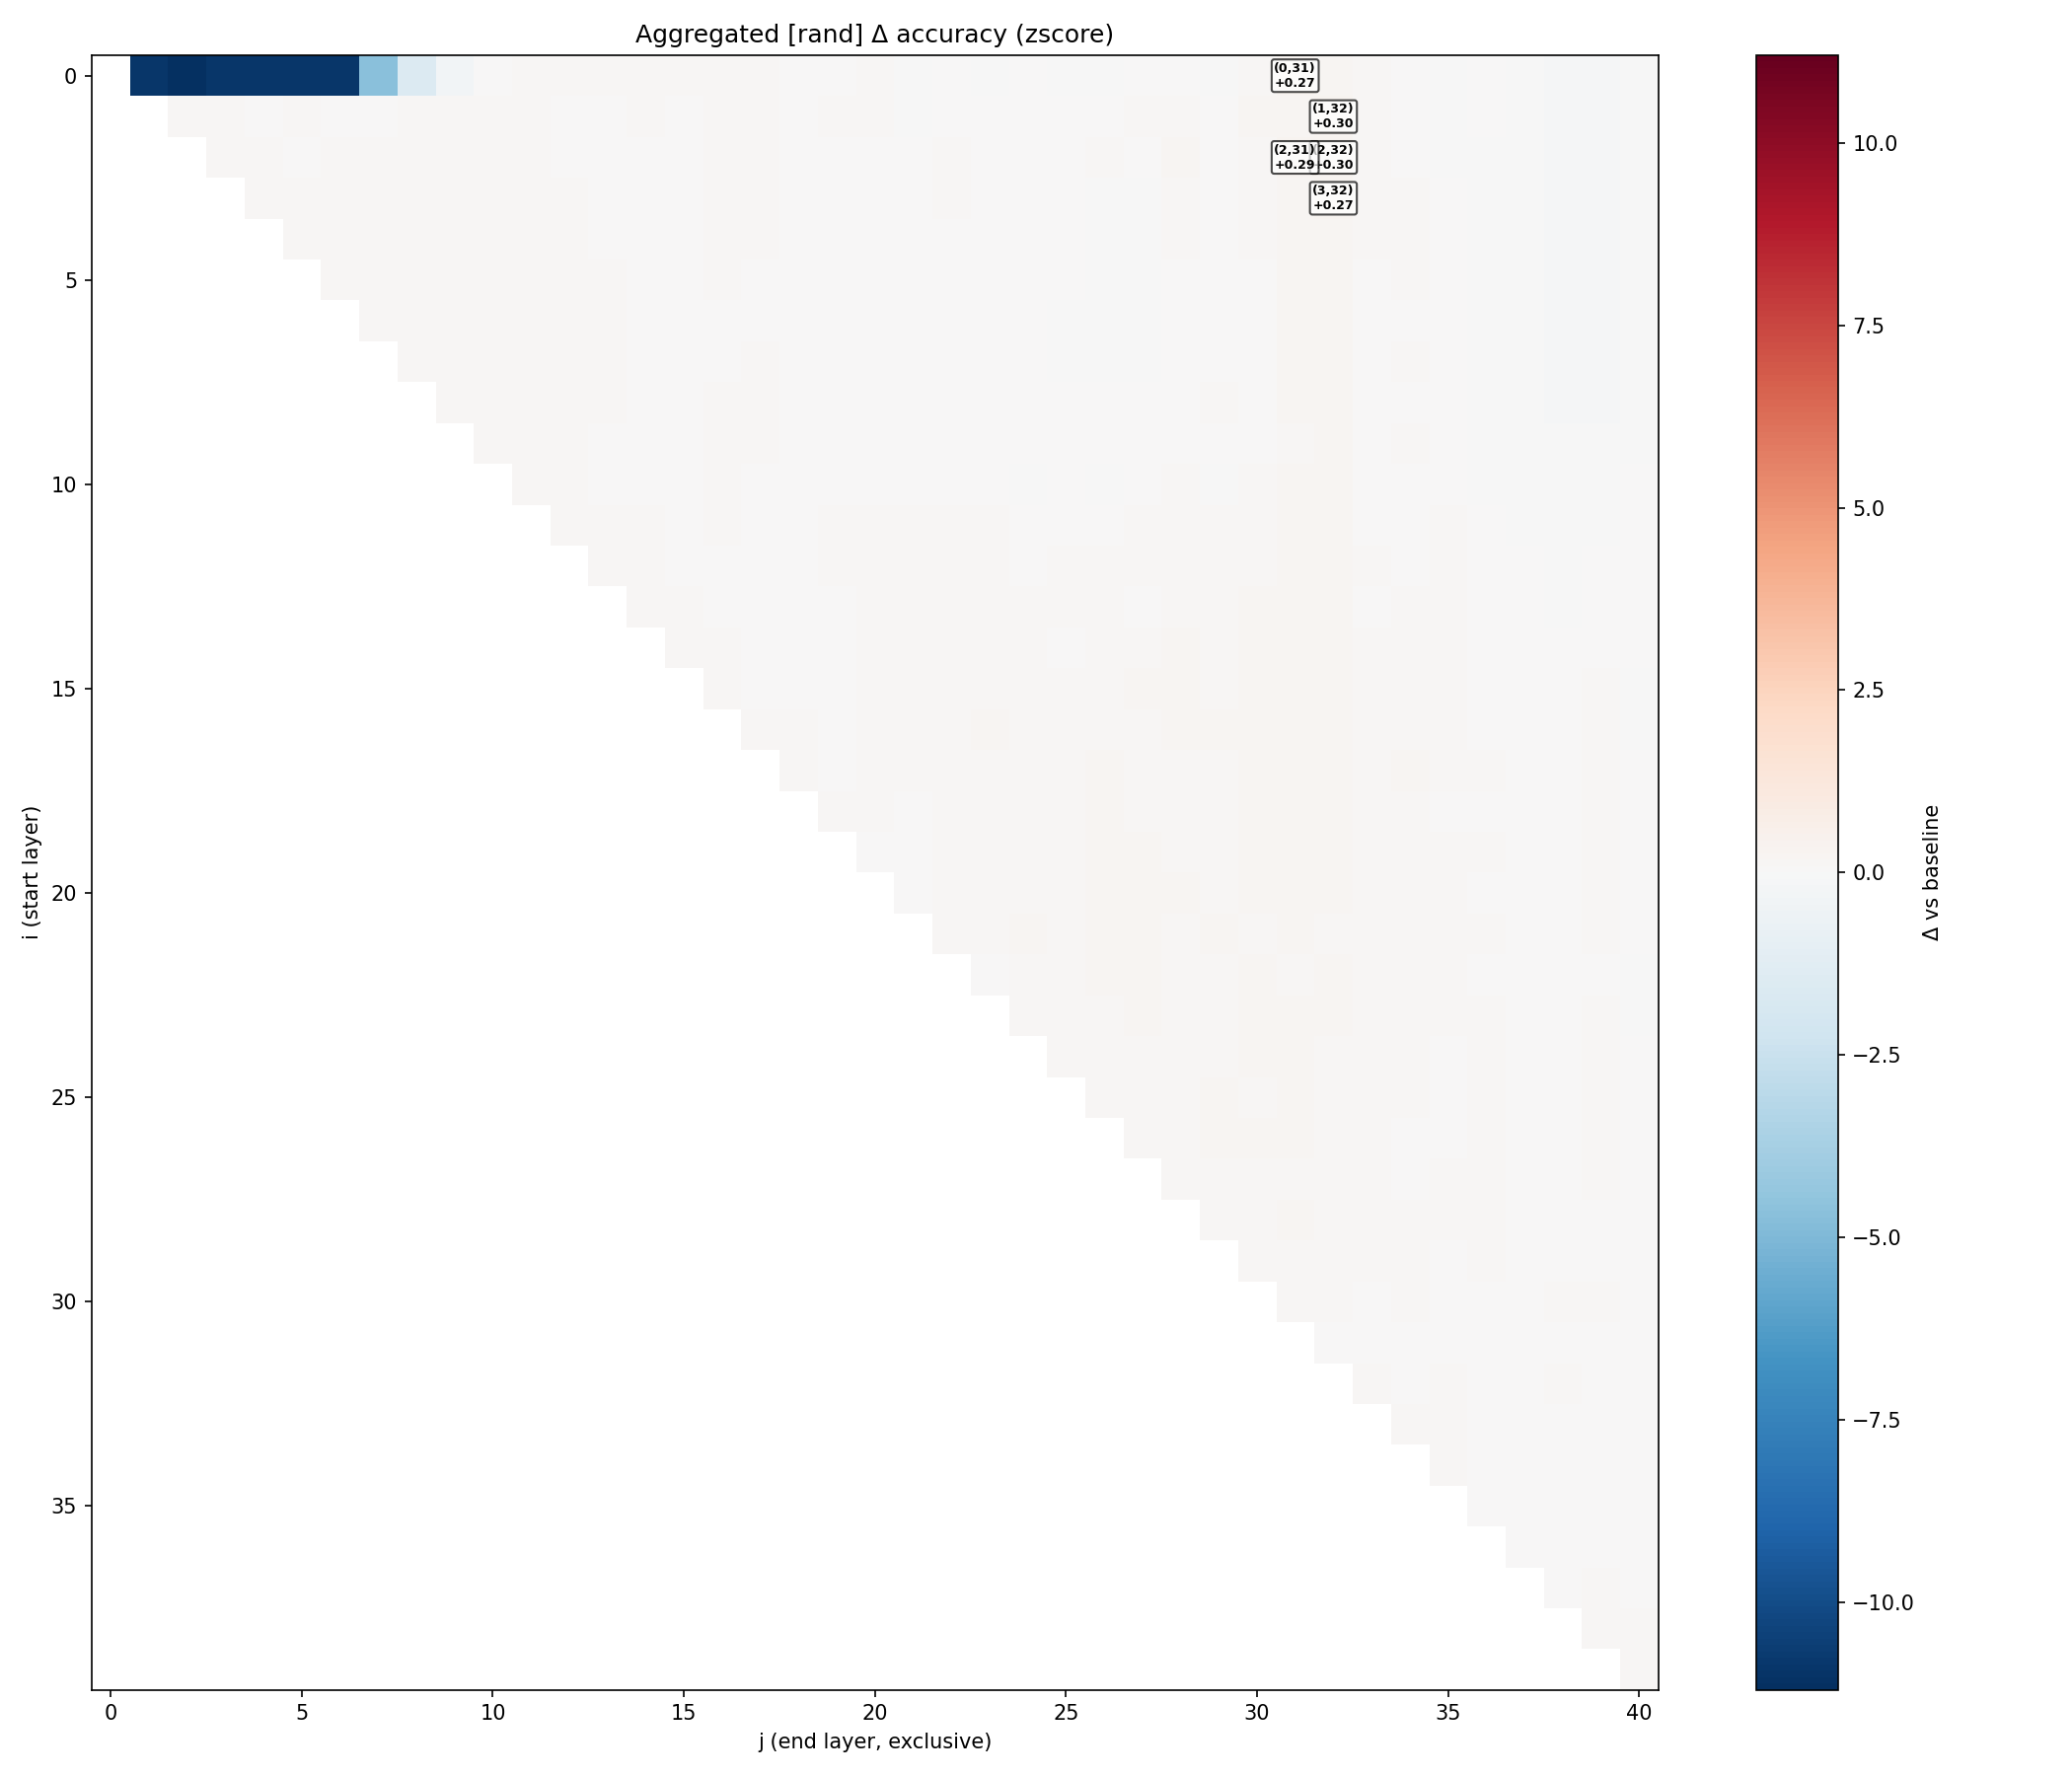
\includegraphics[width=\linewidth]{figures/dino_agg_zscore.png}
\caption{\dino{} (40 layers, 820 configurations)}
\end{subfigure}
\caption{\textbf{Aggregated duplication maps} ($z$-scored $\Delta$accuracy
on the random split, averaged over eleven datasets; red = improvement,
blue = degradation). Row $i$ = first duplicated block; column $j$ =
end of duplicated block (exclusive). Both models show the same
signature: destructive early rows, a broad harmful region for
configurations that begin early and extend deep, and a benign
lower-right (late-start) region carrying faint positive structure.}
\label{fig:heatmaps}
\end{figure}

\begin{figure}[t]
\centering
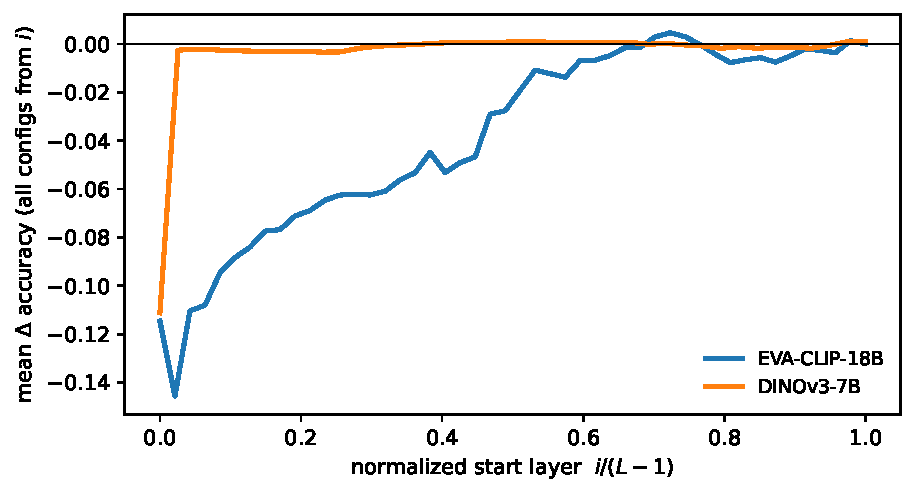
\includegraphics[width=0.54\linewidth]{figures/depth_profile.pdf}
\caption{\textbf{Depth profile of duplication damage.} Mean random-split
$\Delta$accuracy of all configurations starting at layer $i$, averaged
over datasets, against normalized depth. Both models converge to zero
damage as the duplicated region moves toward the output---the reverse of
the LLM profile, where late-layer duplication is catastrophic. \dino{} is
uniformly more tolerant.}
\label{fig:depth}
\end{figure}

\begin{table}[t]
\caption{\textbf{Regional sweep summary} (random split;
$\Delta$accuracy in percentage points). Early: $i < 0.15L$, blocks
shorter than $0.15L$; mid: $i \in [L/3, 2L/3)$, blocks up to $L/4$;
late: $i \ge 0.8L$. Mean/max are over all valid configurations. Per-dataset
values in Appendix~\ref{app:tables}.}
\label{tab:regional}
\centering
\small
\begin{tabular}{lcccc}
\toprule
& \multicolumn{2}{c}{\eva{}} & \multicolumn{2}{c}{\dino{}} \\
\cmidrule(lr){2-3} \cmidrule(lr){4-5}
Region & mean & worst dataset & mean & worst dataset \\
\midrule
Early & $-11.5$ & $-18.8$ (DTD) & $-10.4$ & $-16.4$ (ImageNet) \\
Mid & $-0.9$ & $-4.5$ (same/diff.) & $+0.2$ & $-0.03$ (spatial) \\
Late & $-0.6$ & $-3.8$ (same/diff.) & $-0.1$ & $-1.3$ (counting) \\
\midrule
All-config mean & $-5.8$ & & $-0.7$ & \\
Best single cell & $+18.0$ & (spatial) & $+8.0$ & (counting) \\
Fraction of cells $>0$ & 11.2\% & & 8.1\% & \\
\bottomrule
\end{tabular}
\end{table}

Figures~\ref{fig:heatmaps} and \ref{fig:depth} and
Table~\ref{tab:regional} summarize 21{,}956 configuration--dataset
evaluations. Three regularities hold in \emph{all} 22 dataset--model
combinations:

\textbf{(1) Early layers are duplication-fragile.} Regional means range
from $-2.9$ to $-18.8\pp$; the damage is largest for texture recognition
(DTD, $-18.8\pp$ in \eva{})---precisely the task most dependent on the
low-level statistics early layers compute---and compounds with repetition
count (\S\ref{sec:krepeat}). Duplicating the patch-adjacent machinery
feeds it inputs from the wrong distribution, exactly as the encode-phase
account predicts.

\textbf{(2) Late layers are duplication-immune.} Late-region means are
statistically indistinguishable from zero in both models (largest
magnitude $-1.3\pp$; \dino{}'s late region is $+0.0$ to $+0.06\pp$ on
seven of eleven datasets). This is the mirror image of the LLM result,
where duplicating final layers destroys generation, and it is the
behavioral counterpart of the anatomy finding that \dino{}'s content band
extends to its final layer. Notably \eva{} shows the same immunity
\emph{without} a content band---late-layer tolerance appears to be a
property of encoders as such, not of content-dominant geometry.

\textbf{(3) Nothing large is gained anywhere.} The best single cell in
either sweep is $+18\pp$ (\eva{}, spatial relations, a coherent
neighborhood around $(25\!-\!27, 46\!-\!47)$)---but at $n{=}100$ this is
within reach of the winner's curse, which is what stage two is for.

The global tolerance gap is striking: averaged over every configuration
and dataset, duplication costs \eva{} $-5.8\pp$ and \dino{} $-0.7\pp$.
The self-supervised model's representations pass through a doubled
mid-or-late stack nearly unchanged. We attribute part of this to
\dino{}'s near-ceiling baselines on several probes (its features solve
inside/outside at 99.4\% and symmetry at 99.1\%, versus 83.9\% and
100.0\% for \eva{}; Appendix~\ref{app:tables}), but the gap persists on
datasets with ample headroom (counting: $-0.3$ vs.\ $-5.4\pp$; DTD:
$-0.9$ vs.\ $-5.6\pp$; FGVC: $-0.4$ vs.\ $-10.0\pp$).

\subsection{Selection effects, measured}
\label{sec:selection}

\begin{figure}[t]
\centering
\begin{subfigure}[t]{0.435\linewidth}
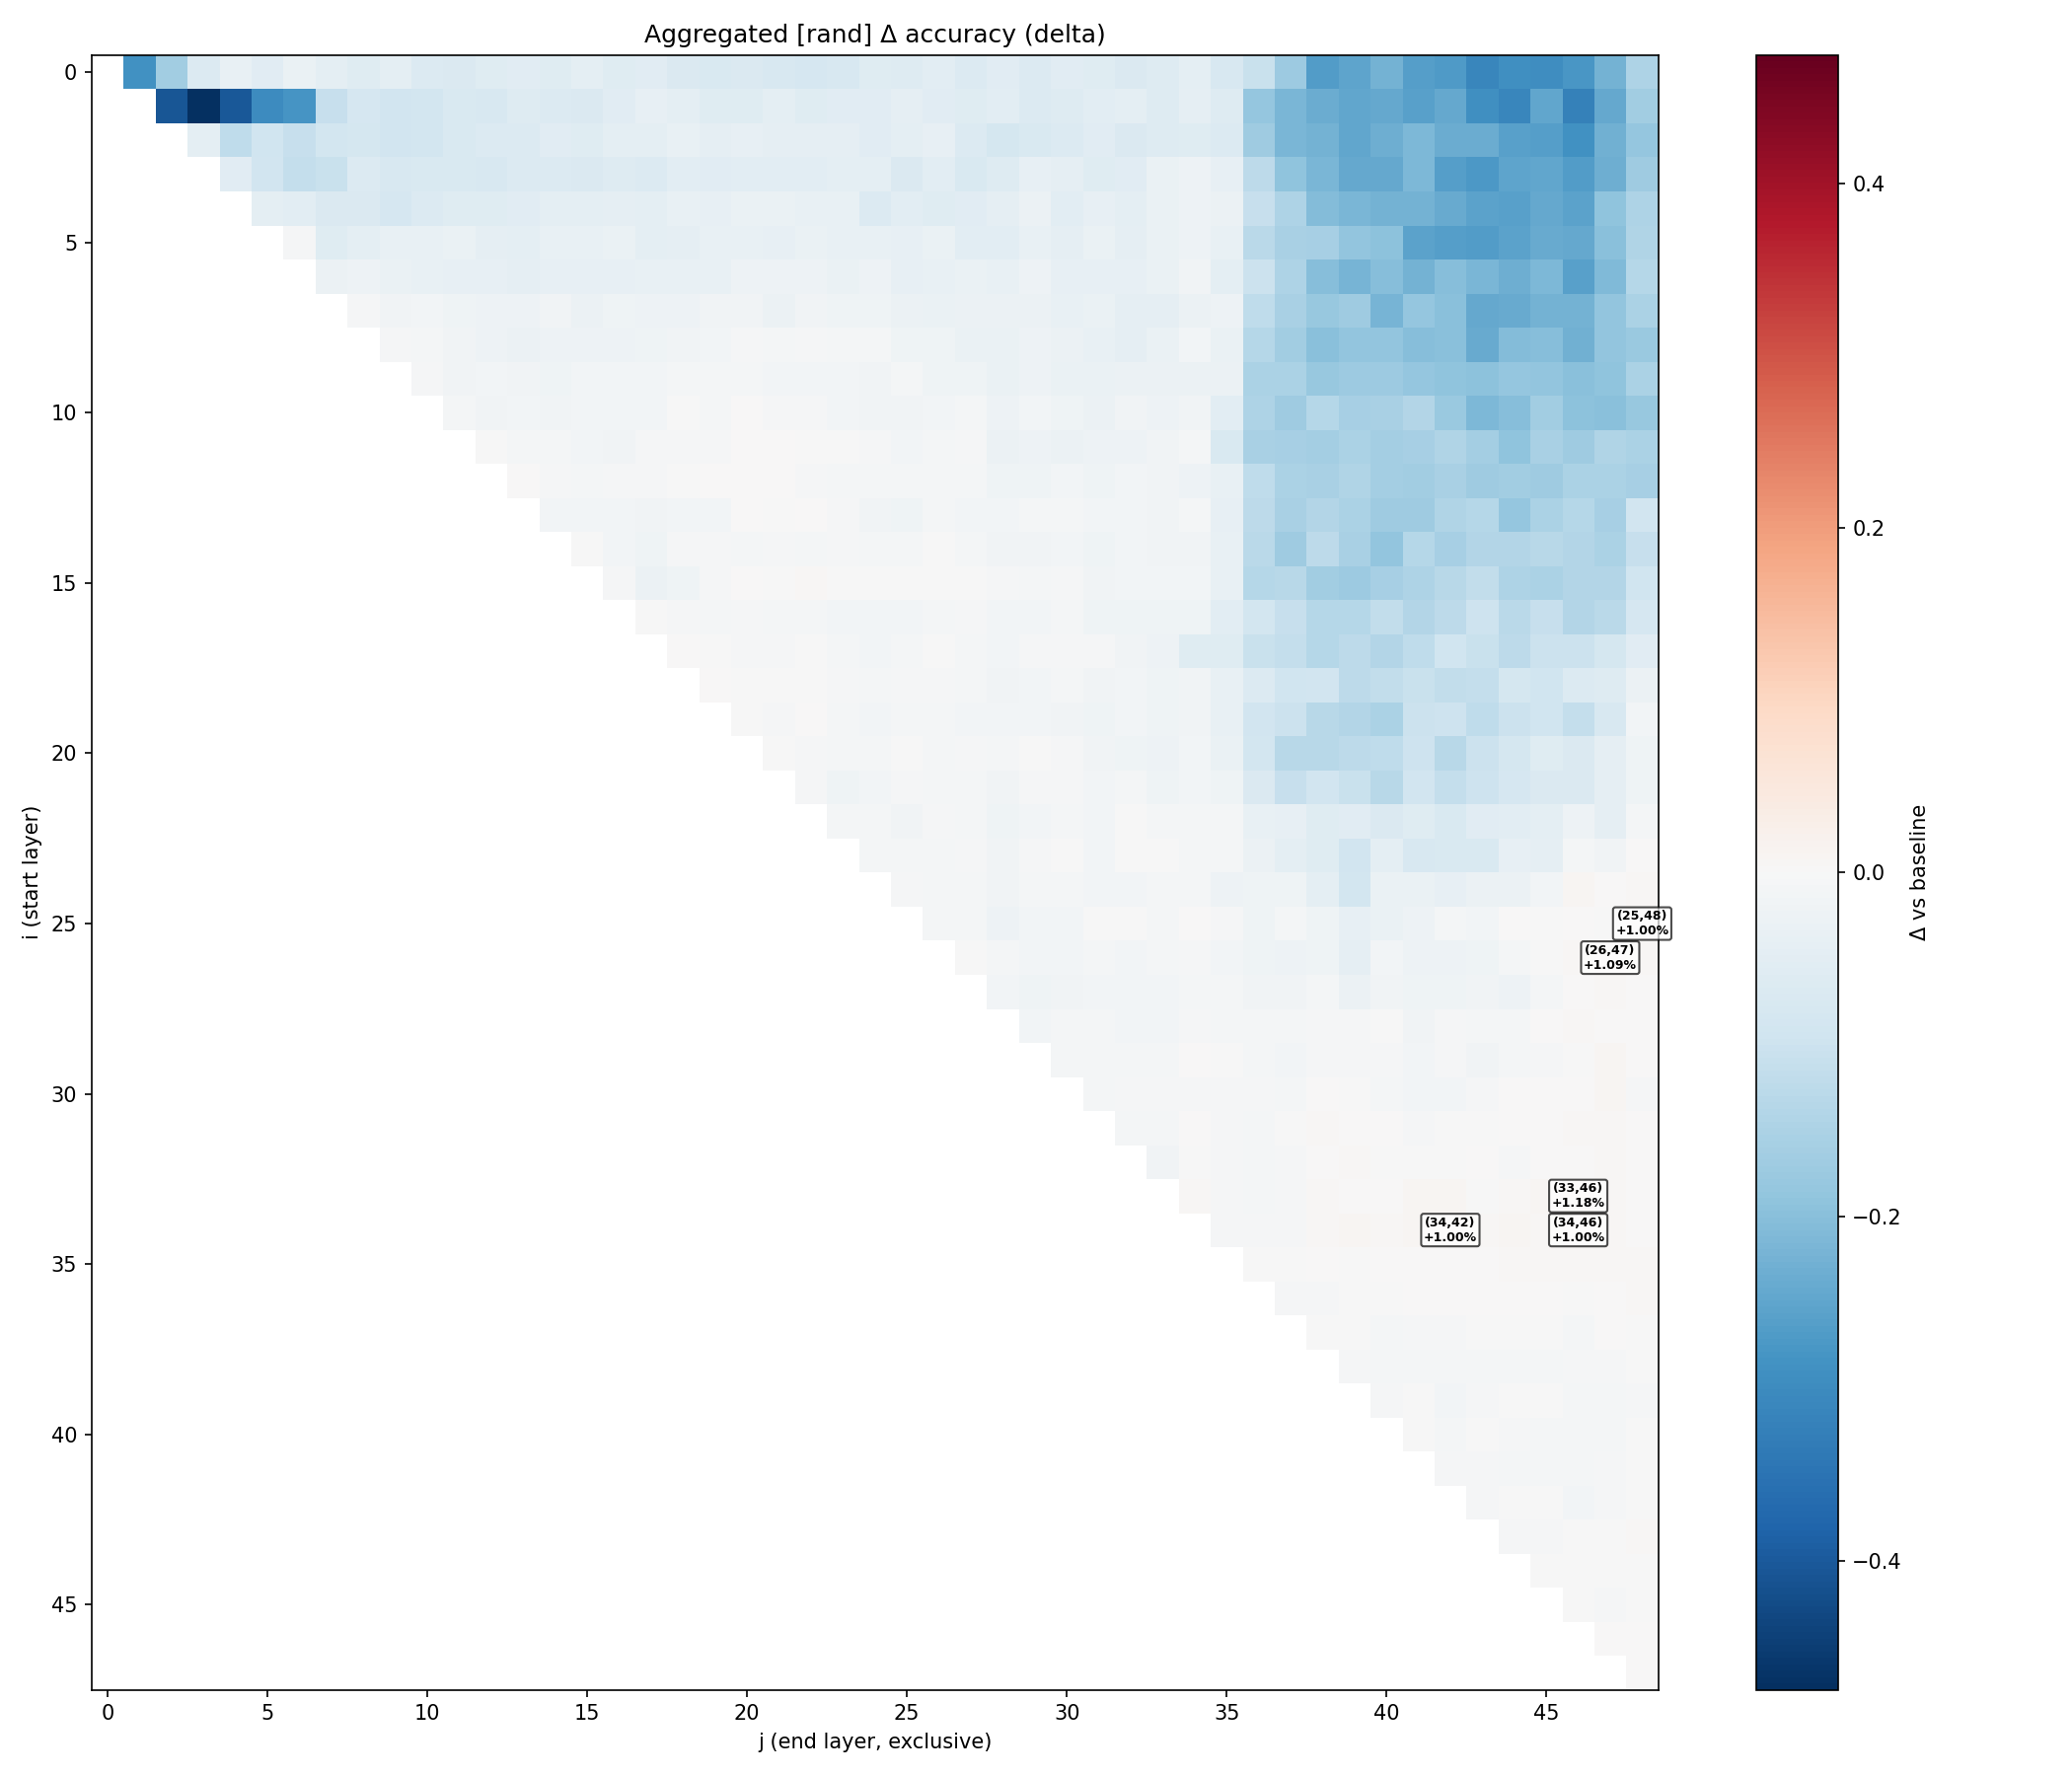
\includegraphics[width=\linewidth]{figures/eva_agg_raw.png}
\caption{Random split (unbiased).}
\end{subfigure}
\hfill
\begin{subfigure}[t]{0.435\linewidth}
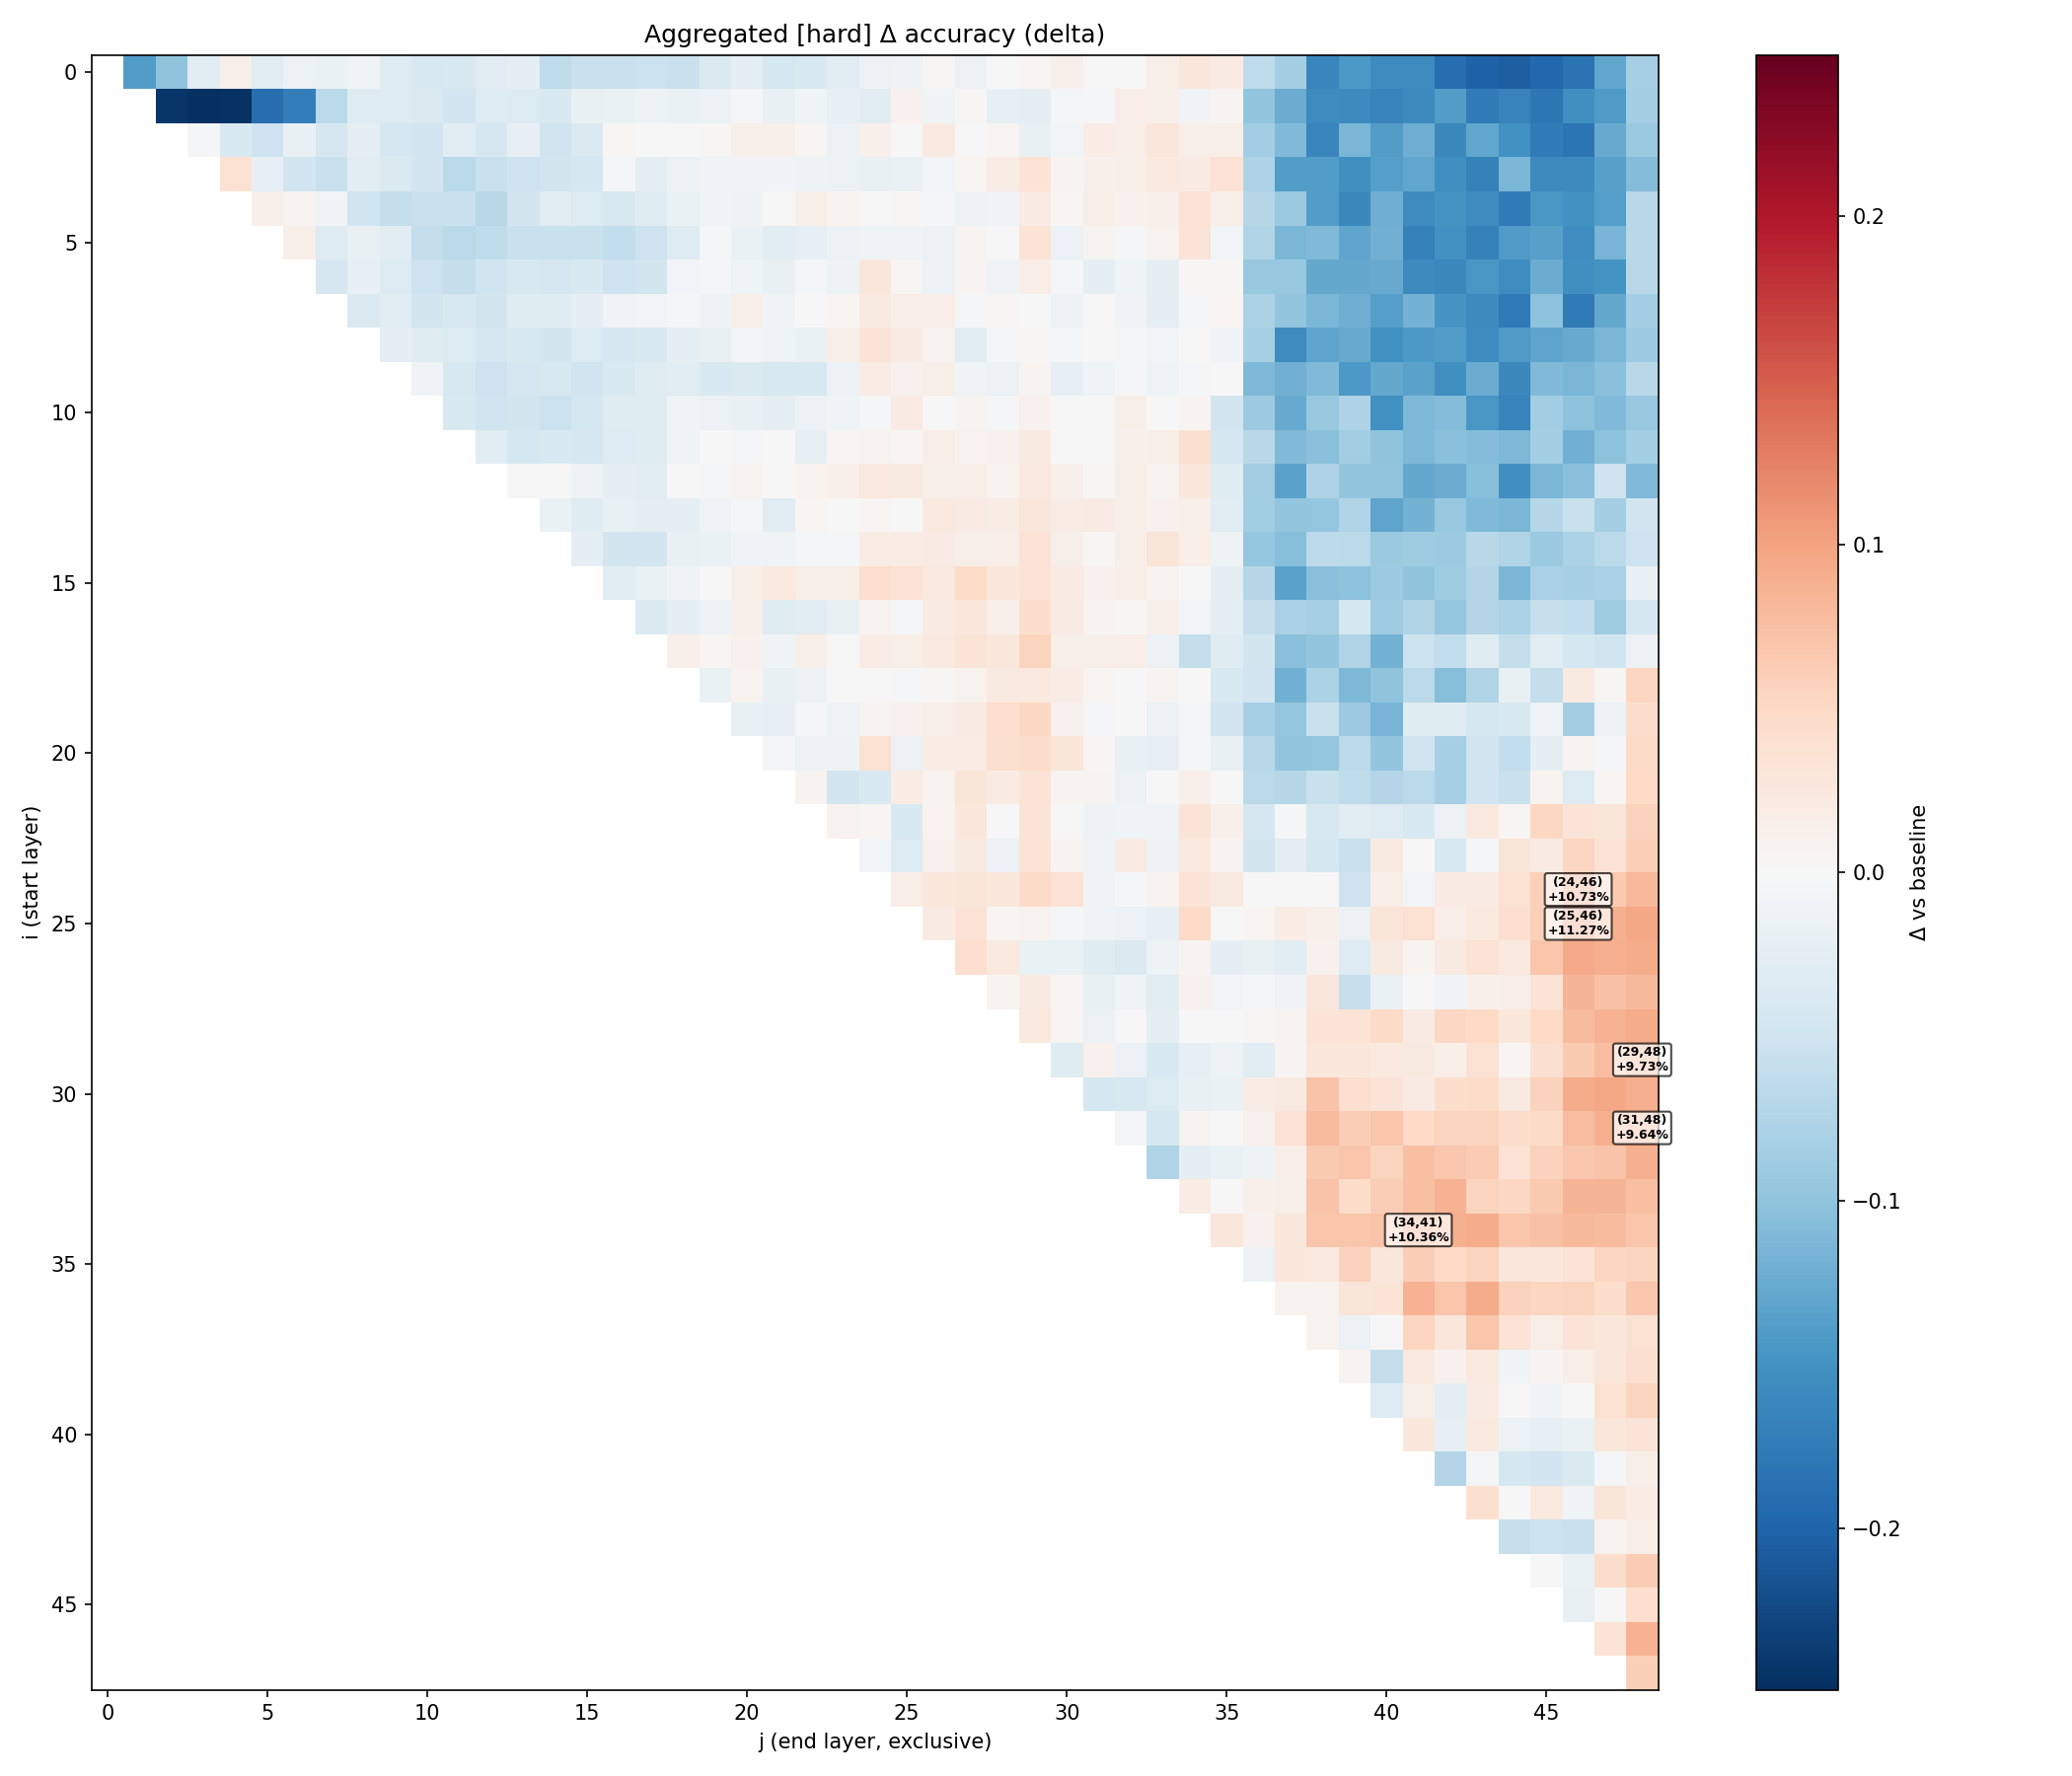
\includegraphics[width=\linewidth]{figures/eva_agg_hard.png}
\caption{Borderline split (selection-sensitive).}
\end{subfigure}
\caption{\textbf{The same interventions, two test splits} (\eva{},
aggregated raw $\Delta$accuracy). The borderline split (right)---whose
images were chosen by their behavior under the baseline model---paints a
systematically rosier picture than the unbiased random split (left):
its sweep maxima reach $+21\pp$ where the random split shows $+4\pp$.
Every conclusion in this paper is drawn from the left panel.}
\label{fig:hardsplit}
\end{figure}

Because the same phenomenon silently inflates any evaluation that selects
test items by baseline behavior, we quantify it directly.
Figure~\ref{fig:hardsplit} contrasts the two test splits on identical
interventions: on the boundary-balanced borderline split, sweep maxima
reach $+21\pp$ (same/different) and $+14\pp$ (EuroSAT), versus $+4\pp$
and $+2\pp$ on the random split---and the pilot design based on
\emph{hardest} images (discarded before any GPU experiment; baseline
accuracy pinned near zero) is more distorted still, since on such a set
\emph{any} perturbation regresses toward the mean. The magnitude of the
gap is worth emphasizing: test-set selection alone manufactures effects
five times larger than anything real in these models. Sweep-style
studies that evaluate on ``the examples the model gets wrong'' inherit
this artifact in full.

\subsection{Stage-two confirmation: no configuration survives}
\label{sec:confirmresults}

\begin{figure}[t]
\centering
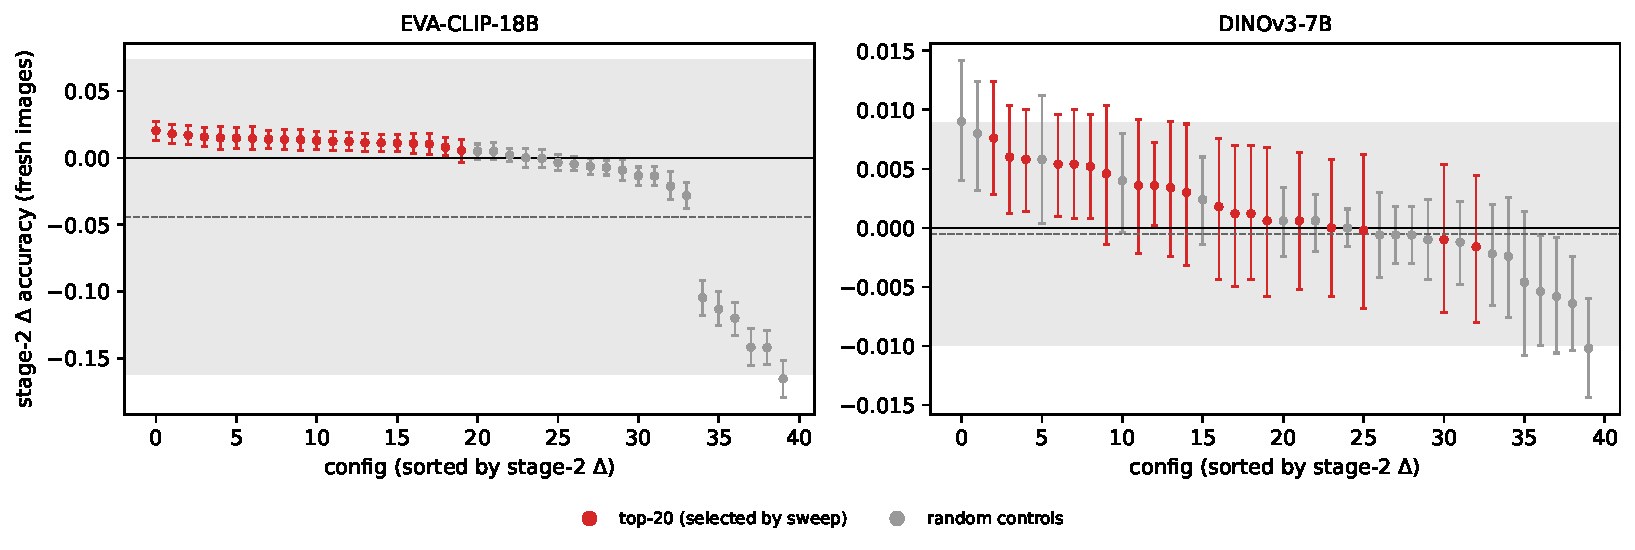
\includegraphics[width=\linewidth]{figures/confirmation.pdf}
\caption{\textbf{Stage-two confirmation on fresh images.} Each point is a
configuration's across-dataset mean $\Delta$accuracy on 500 held-out
images per dataset (bars: 95\% paired-bootstrap CIs); red = top-20 from
the sweep, gray = random controls; shaded band =
$\mu_{\mathrm{ctrl}} \pm 2\sigma_{\mathrm{ctrl}}$. In both models the
selected configurations replicate small positive effects (CIs above
zero) but none clears the pre-specified control band
(Eq.~\ref{eq:criterion}).}
\label{fig:confirm}
\end{figure}

Figure~\ref{fig:confirm} shows the confirmation outcome; full tables are
in Appendix~\ref{app:confirmtables}. For \eva{}, the twenty random
controls average $\mu_{\mathrm{ctrl}} = -4.4\pp$
($\sigma_{\mathrm{ctrl}} = 5.9\pp$)---arbitrary duplication hurts---so
the criterion band sits at $+7.3\pp$. The top-ranked configurations
reproduce positive deltas on fresh images---all twelve leaders have 95\%
CIs excluding zero, led by $(34,41)$ at $+2.0\pp$ $[+1.3, +2.7]$---but
none approaches the band. For \dino{}, controls are tightly concentrated
($\mu_{\mathrm{ctrl}} = -0.05\pp$, $\sigma_{\mathrm{ctrl}} = 0.47\pp$;
random duplication barely hurts this model), the band sits at $+0.9\pp$,
and again no selected configuration clears it; the best is $(14,30)$ at
$+0.76\pp$ $[+0.28, +1.24]$. One control configuration exceeds the band
($+0.90\pp$), consistent with the $\approx 0.5$ false positives expected
among twenty controls at the $2\sigma$ level.

\textbf{Verdict under Eq.~\ref{eq:criterion}: zero confirmed winners in
either model.} We emphasize the two-sided reading. The pre-specified test
asks whether selected configurations beat what \emph{arbitrary}
duplication achieves by luck, and they do not---so claims of
RYS-style circuit gains are not supported. At the same time, the
replication of small positive deltas on held-out data with resampled
references is itself selection-free evidence of a weak, real
second-pass benefit, concentrated in \eva{}'s late-middle stack
(intriguingly, the leader $(34,41)$ is a seven-layer block, the same
width as the original RYS optimum on Qwen2-72B) and \dino{}'s mid-stack.
The effect sizes ($+0.5$--$2\pp$) are an order of magnitude below the
LLM gains that motivated the study.

\subsection{Single-layer $k$-fold repetition}
\label{sec:krepeat}

\begin{figure}[t]
\centering
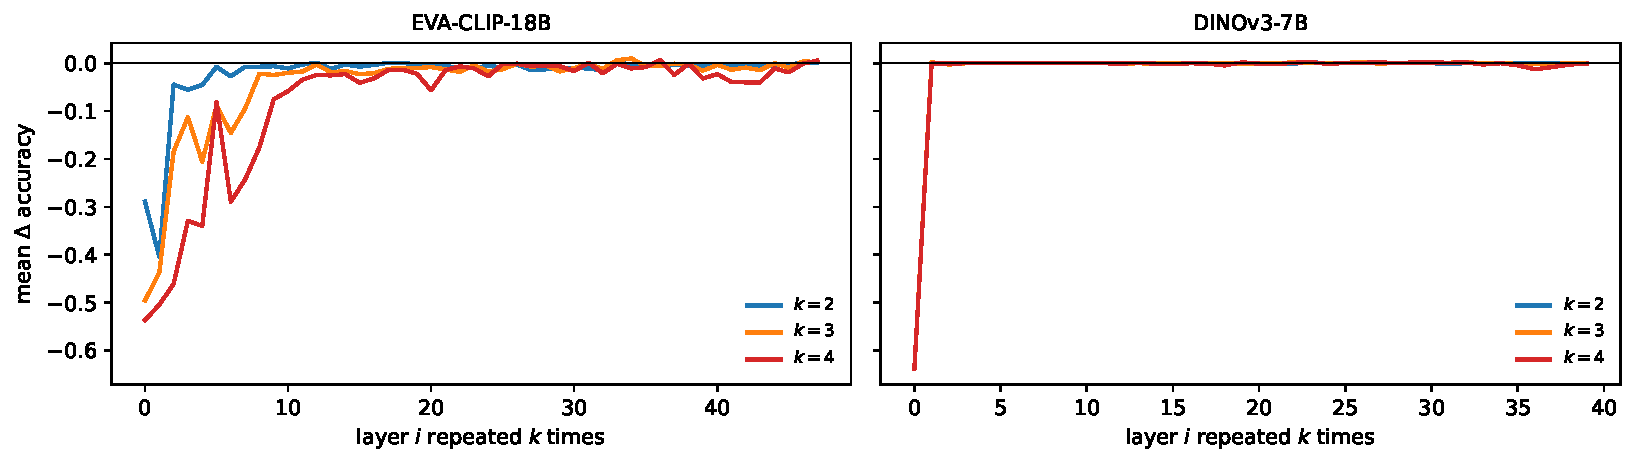
\includegraphics[width=\linewidth]{figures/krepeat.pdf}
\caption{\textbf{Single-layer repetition} (exploratory; no confirmation
stage). Mean random-split $\Delta$accuracy over datasets when layer $i$
is executed $k$ times. Early-layer damage compounds with $k$ in \eva{}
(regional mean $-22\pp$ at $k{=}3$, $-35\pp$ at $k{=}4$) but saturates in
\dino{}; mid- and late-stack repetition remains near-free in both models
even at $k{=}4$.}
\label{fig:krepeat}
\end{figure}

RYS-II reported that repeating a single well-chosen LLM layer three times
yields cheap gains~\citep{hankins2025rysii}. We find no vision analogue
(Figure~\ref{fig:krepeat}): single-layer repetition is neutral at best.
Its depth profile, however, sharpens the sweep's picture. In \eva{},
early-layer damage compounds nearly multiplicatively with $k$
(early-region mean $-22.1\pp$ at $k{=}3$, $-34.8\pp$ at $k{=}4$),
while \dino{}'s early-layer damage saturates ($-10.7\pp$ at both $k$)
and its mid-stack is astonishingly inert ($+0.01\pp$ at $k{=}3$
\emph{and} $k{=}4$): a \dino{} middle layer can be run four times in a
row with no measurable representational consequence.

\subsection{Registered-prediction scorecard}
\label{sec:scorecard}

\begin{table}[t]
\caption{\textbf{Registered predictions versus outcomes.} Predictions
were recorded in the project log before the corresponding sweep results
existed.}
\label{tab:scorecard}
\centering
\small
\begin{tabular}{p{6.2cm}p{6.6cm}}
\toprule
Registered prediction & Outcome \\
\midrule
\eva{}: no content band $\Rightarrow$ duplication broadly harmful, no
beneficial band & \ding{51} Directionally correct, but under-specified:
the harm is strongly depth-structured, not uniform \\
\addlinespace
\dino{}: early layers fragile & \ding{51} Confirmed, all datasets \\
\addlinespace
\dino{}: duplication tolerated within the band (layers 28--40) &
\ding{51} Band deltas $\approx 0.000$; but tolerance is not
band-exclusive---the mid-stack is equally immune, so the band
\emph{under-predicts} the tolerant region \\
\addlinespace
\dino{}: positive effects concentrated in/near the band & \ding{55} The
(small, unconfirmed) positive effects concentrate at
$i \approx 13\!-\!21$, largely \emph{below} the band \\
\bottomrule
\end{tabular}
\end{table}

Table~\ref{tab:scorecard} grades the pre-registered predictions.
Content-dominant geometry correctly identifies \emph{where duplication is
safe} but neither exhausts the tolerant region nor localizes the (weak)
benefits. Representational stability of the kind measured by the anatomy
is evidently necessary-but-coarse: a sufficient account of duplication
tolerance must appeal to more than the content/style organization of the
residual stream.

\section{Discussion}
\label{sec:discussion}

\textbf{Why no reasoning circuits in vision?} The most economical reading
of our negative result combines three observations. First, the LLM gains
arose in \emph{generative, multi-step} inference, where a duplicated
block participates repeatedly in an autoregressive loop and small
per-step refinements can compound; a single-pass encoder offers one
opportunity, and we measure its output geometry directly. Second, the
anatomy shows that the representational precondition identified in
LLMs---a wide format-agnostic band---is absent in the
language-supervised model and thin (six layers, weak gaps) even in the
self-supervised one. Third, where a mild version of the precondition
holds (\dino{}), we observe exactly a mild version of the LLM
phenomenon: perfect tolerance and sub-percentage-point, CI-positive
second-pass effects. Vision transformers may simply sit lower on the same curve: single-pass
objectives exert little pressure to develop computations that profit from
re-execution.

\textbf{The missing decode phase.} The cleanest transferable structure is
the inversion of late-layer behavior. In LLMs the final layers perform
format-specific work whose duplication is catastrophic; in both our
models late-layer duplication is free, and in \dino{} the content band
runs to the final layer. Encoders end \emph{in} representation space.

\textbf{Implications for inference-time depth interventions.} The
duplication maps double as safety maps for the growing family of methods
that manipulate effective depth at inference
time~\citep{schuster2022confident,elhoushi2024layerskip,raposo2024mixture,huang2018multi,yin2022avit}.
Three design rules follow for vision encoders. (i) \emph{The late stack
is a safe surgical region}---the opposite of LLM guidance: layer-level
interventions near the output cost essentially nothing here
($|\Delta| < 0.4\pp$ across 22 dataset--model pairs), whereas LLM
practice treats final layers as untouchable. (ii) \emph{The
patch-adjacent stack is not}: interventions within the first
$\sim$15\% of depth were destructive in every condition we measured, and
the damage compounds super-linearly with repeated application in the
language-supervised model (\S\ref{sec:krepeat}). (iii) \emph{Training
objective modulates the budget}: a self-supervised encoder tolerated
arbitrary mid-stack recycling---four consecutive executions of the same
layer at a measured cost of $+0.01\pp$---suggesting substantially more
zero-shot headroom for skipping, early exit, or iterative refinement
than its language-supervised counterpart, whose whole-map mean cost was
eight times larger. Because duplication (adding a redundant pass) and
deletion (removing a pass)~\citep{lad2024remarkable} stress the same
input-distribution match between adjacent layers, we expect---though we
did not test---these maps to transfer approximately to skipping-style
interventions.

\textbf{Objective, not architecture.} The two arms differ only in
checkpoint; the anatomy differs qualitatively. Language supervision, on
this evidence, prevents the formation of (or masks) appearance-invariant
layer geometry: contrastive image-text training keeps style information
linearly prominent to the last layer, presumably because captions
describe appearance. Self-supervision alone produces the abstraction
gradient. This offers a representational-geometry complement to
behavioral findings on appearance bias~\citep{geirhos2019imagenet} and a
caution for mechanistic claims that generalize across training regimes.

\textbf{Methodological note.} The gap between our sweep-stage leaders
($+18\pp$) and confirmed effects ($\le +2\pp$, below the control band)
quantifies, in a real experiment, how much of an exhaustive-search
leaderboard is selection noise. We commend the two-stage protocol with
random-configuration controls---and the practice of registering
mechanistic predictions before outcome data exist---to future work on
inference-time interventions, where the configuration spaces are large
and the evaluations necessarily small.

\section{Limitations}
\label{sec:limitations}

(1) We probe \emph{representation quality} at the encoder's trained
output interface, not downstream behavior; the original RYS effects were
behavioral. A duplication that improves, e.g., VQA through a
vision-language pipeline without improving nearest-centroid geometry
would escape our measurement (a natural follow-up; Appendix~\ref{app:excluded}).
(2) Datasets are treated as fixed effects and several probes are at or
near ceiling for \dino{}, muting detectable upside there. (3) Two
synthetic probes retain documented residual cues (inside/outside distance
statistics; spatial-relation absolute position), and one (symmetry) is at
ceiling for both models. (4) The anatomy stimuli are procedural; for a
contrastive model, style is arguably legitimate content, which our
objective-ablation design addresses but does not eliminate. (5) Two
models, one run each (deterministic inference); conclusions are about
these checkpoints and scales.

\section{Conclusion}
\label{sec:conclusion}

We performed the first exhaustive layer-duplication study in vision
transformers, at the largest openly available scales, under a
selection-robust, pre-registered protocol. Inference-time layer
duplication does not buy vision what it bought language models: no
configuration among 1{,}996 produces confirmed gains in either a
language-supervised or a self-supervised frontier ViT. What the
intervention reveals instead is structure: a universal early-layer
fragility, a late-layer immunity that inverts the LLM picture and follows
from encoders' lack of a decode phase, a content-dominant band that
exists only without language supervision, and a small but replicable
second-pass benefit that hints the LLM phenomenon has a faint visual
shadow. All artifacts required to reproduce or extend every number and
figure in this paper are public.

\section*{Reproducibility statement}

Code, the complete decision log (\texttt{docs/methods.md}), all score
matrices, per-image outcomes, probe-set indices, anatomy features, and
generated figures are available at \url{https://github.com/avchadha/rys}
(raw data on the \texttt{results-sync} branch). Every stochastic choice
is seeded; dataset stimuli for the synthetic probes and anatomy grid are
regenerable from code. Hardware and cost: one NVIDIA H100 80GB
(Lambda Cloud); $\sim$27.5 h for the \eva{} arm, $\sim$6 h for the
\dino{} arm, $\approx$\$95 total. Software pins and verified
checkpoint-interface facts are listed in Appendix~\ref{app:repro}.

\bibliographystyle{plainnat}
\bibliography{references}

\clearpage
\appendix

\section{Task battery details}
\label{app:synthetic}

\subsection{Real-world datasets}
ImageNet-1k and Places365 are subsampled to 100 classes each
(deterministic seed) to equalize probe cost; all other datasets use their
full label sets (DTD 47, EuroSAT 10, Stanford~40 40, FGVC-Aircraft 100).
Images pass through each model's native $224{\times}224$ preprocessing.

\subsection{Synthetic visual-reasoning probes}
All probes are generated procedurally at $448{\times}448$ (downscaled by
the model transform), with disjoint generation seeds for
reference/candidate pools, and are regenerable exactly from code. Each
was adversarially reviewed for shortcut cues; the shipped versions
include the following controls:

\textbf{Counting} (10 classes; 1--10 dots). Radii drawn i.i.d.\
$\mathcal{U}\{12..40\}$ \emph{before} placement (count-independent size
distribution); positions rejection-sampled for strict non-overlap
($\ge 6$px gap) with whole-layout restart on failure, so visible count
always equals the label. Residual cue: total colored area correlates with
count (inherent to numerosity stimuli).

\textbf{Same/different} (2 classes). Two polygons; ``same'' pairs share
the vertex set, translated and rotated $\pm 0.6$\,rad; ``different''
pairs use a fresh polygon with the same vertex count, rescaled to match
the reference polygon's area exactly. Colors always differ between the
two shapes.

\textbf{Spatial relation} (4 classes). Red reference disc jittered
$\pm 70$px around center; blue triangle at gap 80--160px with $\pm 25$px
cross-axis jitter. Residual cue: absolute position retains partial
information (jitter is smaller than the maximum gap).

\textbf{Symmetry} (2 classes). Mirror-symmetric versus scrambled dot
patterns; scrambled images reuse the mirrored dots' exact (y, radius,
color) multiset and resample only x, so per-half color histograms, size
distributions, and vertical marginals are identical between classes.

\textbf{Inside/outside} (2 classes). Irregular star-shaped contour
(6--12 vertices, radii $0.6$--$1.0R$, $R \in [100,160]$) drawn as
outline; the query dot must clear the boundary by a visible margin and
lie in a distance annulus where both classes occur; contours are
regenerated when placement is infeasible; ray casting provides ground
truth. Residual cue: distance-from-center separates the classes
partially (weakened, not eliminated).

\subsection{Excluded designs}
\label{app:excluded}
Vision-language models were excluded because (i) their vision towers are
small relative to the models studied here (Qwen2.5-VL uses a
$\sim$0.7B-parameter ViT across its 3B--72B family), and (ii) measuring
duplication through an LLM confounds representational change with the
LLM's tolerance to off-distribution visual tokens. Applying the
best/worst configurations found here to a VLM's vision tower and
measuring task behavior is the natural behavioral follow-up. CLEVR and
additional fine-grained natural-photo datasets were excluded as
redundant with existing battery members; beam-searched multi-block
compositions and surrogate-model search~\citep{hankins2025rysii} were
excluded because the configuration space is exhaustively enumerable at
these depths.

\section{Probe methodology details}
\label{app:probemeth}

\subsection{Borderline split construction}
\label{app:selection}
For each dataset, 1{,}000 candidate images are drawn from the test split
(restricted to the class subset). Under baseline features, each candidate
receives a margin $m = s_{\mathrm{true}} - \max_{c \ne \mathrm{true}}
s_c$ (cosine similarities to class centroids). The borderline split
comprises the 50 misclassified candidates with margin closest to zero
and the 50 correctly classified candidates with margin closest to zero.
The random split is drawn uniformly from the remaining candidates.
Selecting instead the \emph{most negative} margins (the original plan,
discarded before any GPU experiments) pins baseline accuracy near zero
and produces guaranteed-positive deltas under any perturbation. The
empirical comparison is quantified in the main text
(\S\ref{sec:selection}, Figure~\ref{fig:hardsplit}).

\subsection{Aggregation}
\label{app:agg}
Per-dataset $\Delta$ matrices are aggregated two ways: an unweighted mean
(interpretable units) and a mean of per-dataset $z$-scores, where each
dataset's deltas are standardized over its own valid cells. The $z$-scored
random-split accuracy matrix is the canonical ranking object; it prevents
high-variance binary probes from dominating the mean.

\subsection{Noise null}
Gaussian noise with per-dimension standard deviation
$\alpha \, \overline{\lVert f \rVert} / \sqrt{D}$ is added to reference
and test features simultaneously, $\alpha \in \{0.005, 0.01, 0.02, 0.05,
0.1\}$, 20 seeds each; the maximum mean $\Delta$accuracy across
magnitudes is reported per dataset in
Tables~\ref{tab:evadatasets}--\ref{tab:dinodatasets}. This null is
deliberately weak (duplication shifts features coherently, not
isotropically); the matched null is the random-configuration control of
the confirmation stage.

\subsection{Bootstrap}
Per-image correctness bitmaps are persisted for every (configuration,
dataset, split). CIs are percentile intervals from 2{,}000 paired
bootstrap resamples over images within each dataset, with per-dataset
deltas averaged across datasets in each resample
\citep{efron1994introduction}. Datasets are fixed effects; CIs are
conditional on the reference sets (stage two resamples them).

\section{Anatomy stimulus grid}
\label{app:grid}

\begin{figure}[h]
\centering
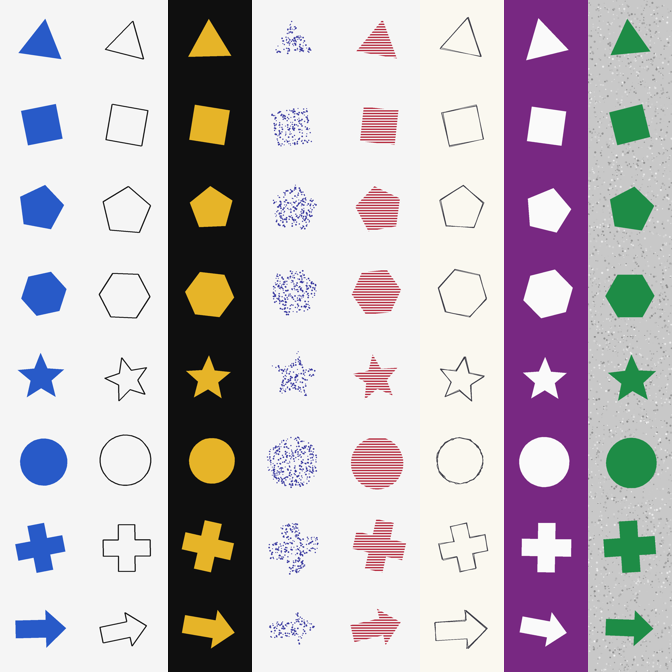
\includegraphics[width=0.6\linewidth]{figures/style_content_grid.png}
\caption{\textbf{The $8{\times}8$ style-by-content grid} (one jitter
instance shown per cell). Rows: shape classes (triangle, square,
pentagon, hexagon, star, circle, cross, arrow). Columns: rendering styles
(solid-on-white, outline, solid-on-black, stippled, striped, sketch,
inverted, cluttered background).}
\label{fig:grid}
\end{figure}

Shapes are defined as canonical vertex geometry and rendered at radius
$\approx 140$px on a $448{\times}448$ canvas. Per-instance jitter
(rotation $\pm 15^{\circ}$, translation $\pm 12$px, scale
$\times 0.85$--$1.0$) defeats pixel-level matching between same-shape
pairs while preserving unambiguous shape identity; larger rotations were
rejected because they corrupt content labels (a square at $45^{\circ}$ is
a diamond). Two instances per cell yield 128 images and add a
same-content-same-style ceiling category. With category counts 896 /
896 / 6{,}272 / 64 (same-content, same-style, different, ceiling), the
three primary curves average over hundreds of pairs per layer.

\section{Full result tables}
\label{app:tables}

\begin{table}[h]
\caption{\textbf{\eva{} per-dataset summary} (random split; accuracies as
fractions, deltas in fractions of accuracy). Border/rand: baseline
accuracy on the borderline/random split. Noise: maximum mean
$\Delta$accuracy under the Gaussian null. Mean/max over all 1{,}176
configurations; early/mid/late as in Table~\ref{tab:regional}.}
\label{tab:evadatasets}
\centering
\scriptsize
\setlength{\tabcolsep}{3.4pt}
\begin{tabular}{lrrrrrrrrrrr}
\toprule
Dataset & Cls & Refs & Cand & Border & Rand & Noise & Mean & Max & Early & Mid & Late \\
\midrule
counting & 10 & 150 & .392 & .500 & .390 & $+.000$ & $-.054$ & $+.070$ & $-.033$ & $-.013$ & $+.006$ \\
DTD & 47 & 235 & .684 & .500 & .750 & $+.006$ & $-.056$ & $+.030$ & $-.188$ & $-.001$ & $-.004$ \\
EuroSAT & 10 & 150 & .899 & .500 & .930 & $+.000$ & $-.069$ & $+.020$ & $-.150$ & $-.003$ & $-.001$ \\
FGVC-Aircraft & 100 & 500 & .691 & .500 & .730 & $+.000$ & $-.100$ & $+.030$ & $-.132$ & $-.014$ & $-.004$ \\
ImageNet-100 & 100 & 500 & .925 & .500 & .960 & $+.002$ & $-.047$ & $+.010$ & $-.163$ & $-.001$ & $-.002$ \\
inside/outside & 2 & 100 & .839 & .500 & .900 & $+.009$ & $-.062$ & $+.060$ & $-.029$ & $-.017$ & $-.002$ \\
Places365-100 & 100 & 500 & .587 & .500 & .600 & $+.000$ & $-.062$ & $+.040$ & $-.120$ & $-.006$ & $-.011$ \\
same/different & 2 & 100 & .711 & .500 & .820 & $+.007$ & $-.102$ & $+.040$ & $-.128$ & $-.045$ & $-.038$ \\
spatial relation & 4 & 152 & .818 & .500 & .800 & $+.004$ & $-.033$ & $+.180$ & $-.060$ & $-.002$ & $-.002$ \\
Stanford~40 & 40 & 200 & .862 & .500 & .920 & $+.008$ & $-.042$ & $+.040$ & $-.111$ & $+.000$ & $-.004$ \\
symmetry & 2 & 100 & 1.000 & 1.000 & 1.000 & $+.000$ & $-.016$ & $+.000$ & $-.048$ & $+.000$ & $+.000$ \\
\bottomrule
\end{tabular}
\end{table}

\begin{table}[h]
\caption{\textbf{\dino{} per-dataset summary} (columns as in
Table~\ref{tab:evadatasets}; 820 configurations). Note the near-ceiling
baselines on the geometric probes and ImageNet, and the dramatically
smaller whole-matrix means.}
\label{tab:dinodatasets}
\centering
\scriptsize
\setlength{\tabcolsep}{3.4pt}
\begin{tabular}{lrrrrrrrrrrr}
\toprule
Dataset & Cls & Refs & Cand & Border & Rand & Noise & Mean & Max & Early & Mid & Late \\
\midrule
counting & 10 & 150 & .430 & .500 & .420 & $+.000$ & $-.003$ & $+.080$ & $-.057$ & $+.014$ & $-.013$ \\
DTD & 47 & 235 & .695 & .500 & .750 & $+.000$ & $-.009$ & $+.020$ & $-.118$ & $+.004$ & $+.001$ \\
EuroSAT & 10 & 150 & .891 & .500 & .950 & $+.011$ & $-.011$ & $+.000$ & $-.137$ & $-.000$ & $+.000$ \\
FGVC-Aircraft & 100 & 500 & .492 & .500 & .450 & $+.009$ & $-.004$ & $+.020$ & $-.075$ & $+.000$ & $-.001$ \\
ImageNet-100 & 100 & 500 & .935 & .500 & .990 & $-.000$ & $-.010$ & $+.010$ & $-.164$ & $+.000$ & $+.000$ \\
inside/outside & 2 & 100 & .994 & .940 & 1.000 & $+.000$ & $-.003$ & $+.000$ & $-.077$ & $+.000$ & $+.000$ \\
Places365-100 & 100 & 500 & .555 & .500 & .610 & $+.003$ & $-.009$ & $+.020$ & $-.097$ & $+.000$ & $+.001$ \\
same/different & 2 & 100 & .830 & .500 & .930 & $+.025$ & $-.001$ & $+.020$ & $-.080$ & $+.001$ & $+.000$ \\
spatial relation & 4 & 152 & .938 & .500 & .990 & $-.000$ & $-.008$ & $+.000$ & $-.113$ & $-.000$ & $+.000$ \\
Stanford~40 & 40 & 200 & .886 & .500 & .960 & $+.018$ & $-.011$ & $+.000$ & $-.158$ & $+.000$ & $+.000$ \\
symmetry & 2 & 100 & .991 & .910 & 1.000 & $+.000$ & $-.004$ & $+.000$ & $-.098$ & $+.000$ & $+.000$ \\
\bottomrule
\end{tabular}
\end{table}

\begin{table}[h]
\caption{\textbf{Stage-two confirmation, leading configurations.} Deltas
are across-dataset means on 500 fresh images per dataset with resampled
reference sets; brackets: 95\% paired-bootstrap CIs. ``Beats null'':
Eq.~\ref{eq:criterion}. Controls: \eva{}
$\mu = -.0441$, $\sigma = .0586$; \dino{} $\mu = -.0005$,
$\sigma = .0047$.}
\label{tab:confirm}
\centering
\scriptsize
\begin{tabular}{lrlc@{\hskip 26pt}lrlc}
\toprule
\multicolumn{4}{c}{\eva{}} & \multicolumn{4}{c}{\dino{}} \\
\cmidrule(r{22pt}){1-4} \cmidrule(l){5-8}
Config & $\Delta$ & CI & Beats & Config & $\Delta$ & CI & Beats \\
\midrule
(34, 41) & $+.0204$ & $[+.0132, +.0272]$ & no & (13, 28)$^{c}$ & $+.0090$ & $[+.0040, +.0142]$ & yes$^{*}$ \\
(34, 44) & $+.0180$ & $[+.0108, +.0250]$ & no & (16, 28)$^{c}$ & $+.0080$ & $[+.0032, +.0124]$ & no \\
(34, 42) & $+.0170$ & $[+.0100, +.0242]$ & no & (14, 30) & $+.0076$ & $[+.0028, +.0124]$ & no \\
(33, 41) & $+.0156$ & $[+.0084, +.0228]$ & no & (13, 31) & $+.0060$ & $[+.0012, +.0104]$ & no \\
(25, 48) & $+.0150$ & $[+.0062, +.0234]$ & no & (20, 27) & $+.0058$ & $[+.0014, +.0100]$ & no \\
(30, 47) & $+.0148$ & $[+.0072, +.0224]$ & no & (13, 26)$^{c}$ & $+.0058$ & $[+.0004, +.0112]$ & no \\
(24, 48) & $+.0144$ & $[+.0060, +.0234]$ & no & (21, 27) & $+.0054$ & $[+.0010, +.0096]$ & no \\
(34, 46) & $+.0140$ & $[+.0072, +.0204]$ & no & (15, 31) & $+.0054$ & $[+.0008, +.0100]$ & no \\
(33, 44) & $+.0138$ & $[+.0066, +.0212]$ & no & (16, 31) & $+.0052$ & $[+.0008, +.0096]$ & no \\
(29, 47) & $+.0136$ & $[+.0058, +.0214]$ & no & (4, 31) & $+.0046$ & $[-.0014, +.0104]$ & no \\
\bottomrule
\multicolumn{8}{l}{$^{c}$random control configuration. $^{*}$one
control exceeding the band matches the expected $2\sigma$ false-positive}\\
\multicolumn{8}{l}{rate among twenty controls ($\approx 0.5$); no
\emph{selected} configuration meets the criterion in either model.}
\end{tabular}
\label{app:confirmtables}
\end{table}

\section{Additional figures}
\label{app:figures}

\begin{figure}[h]
\centering
\begin{subfigure}[t]{0.33\linewidth}
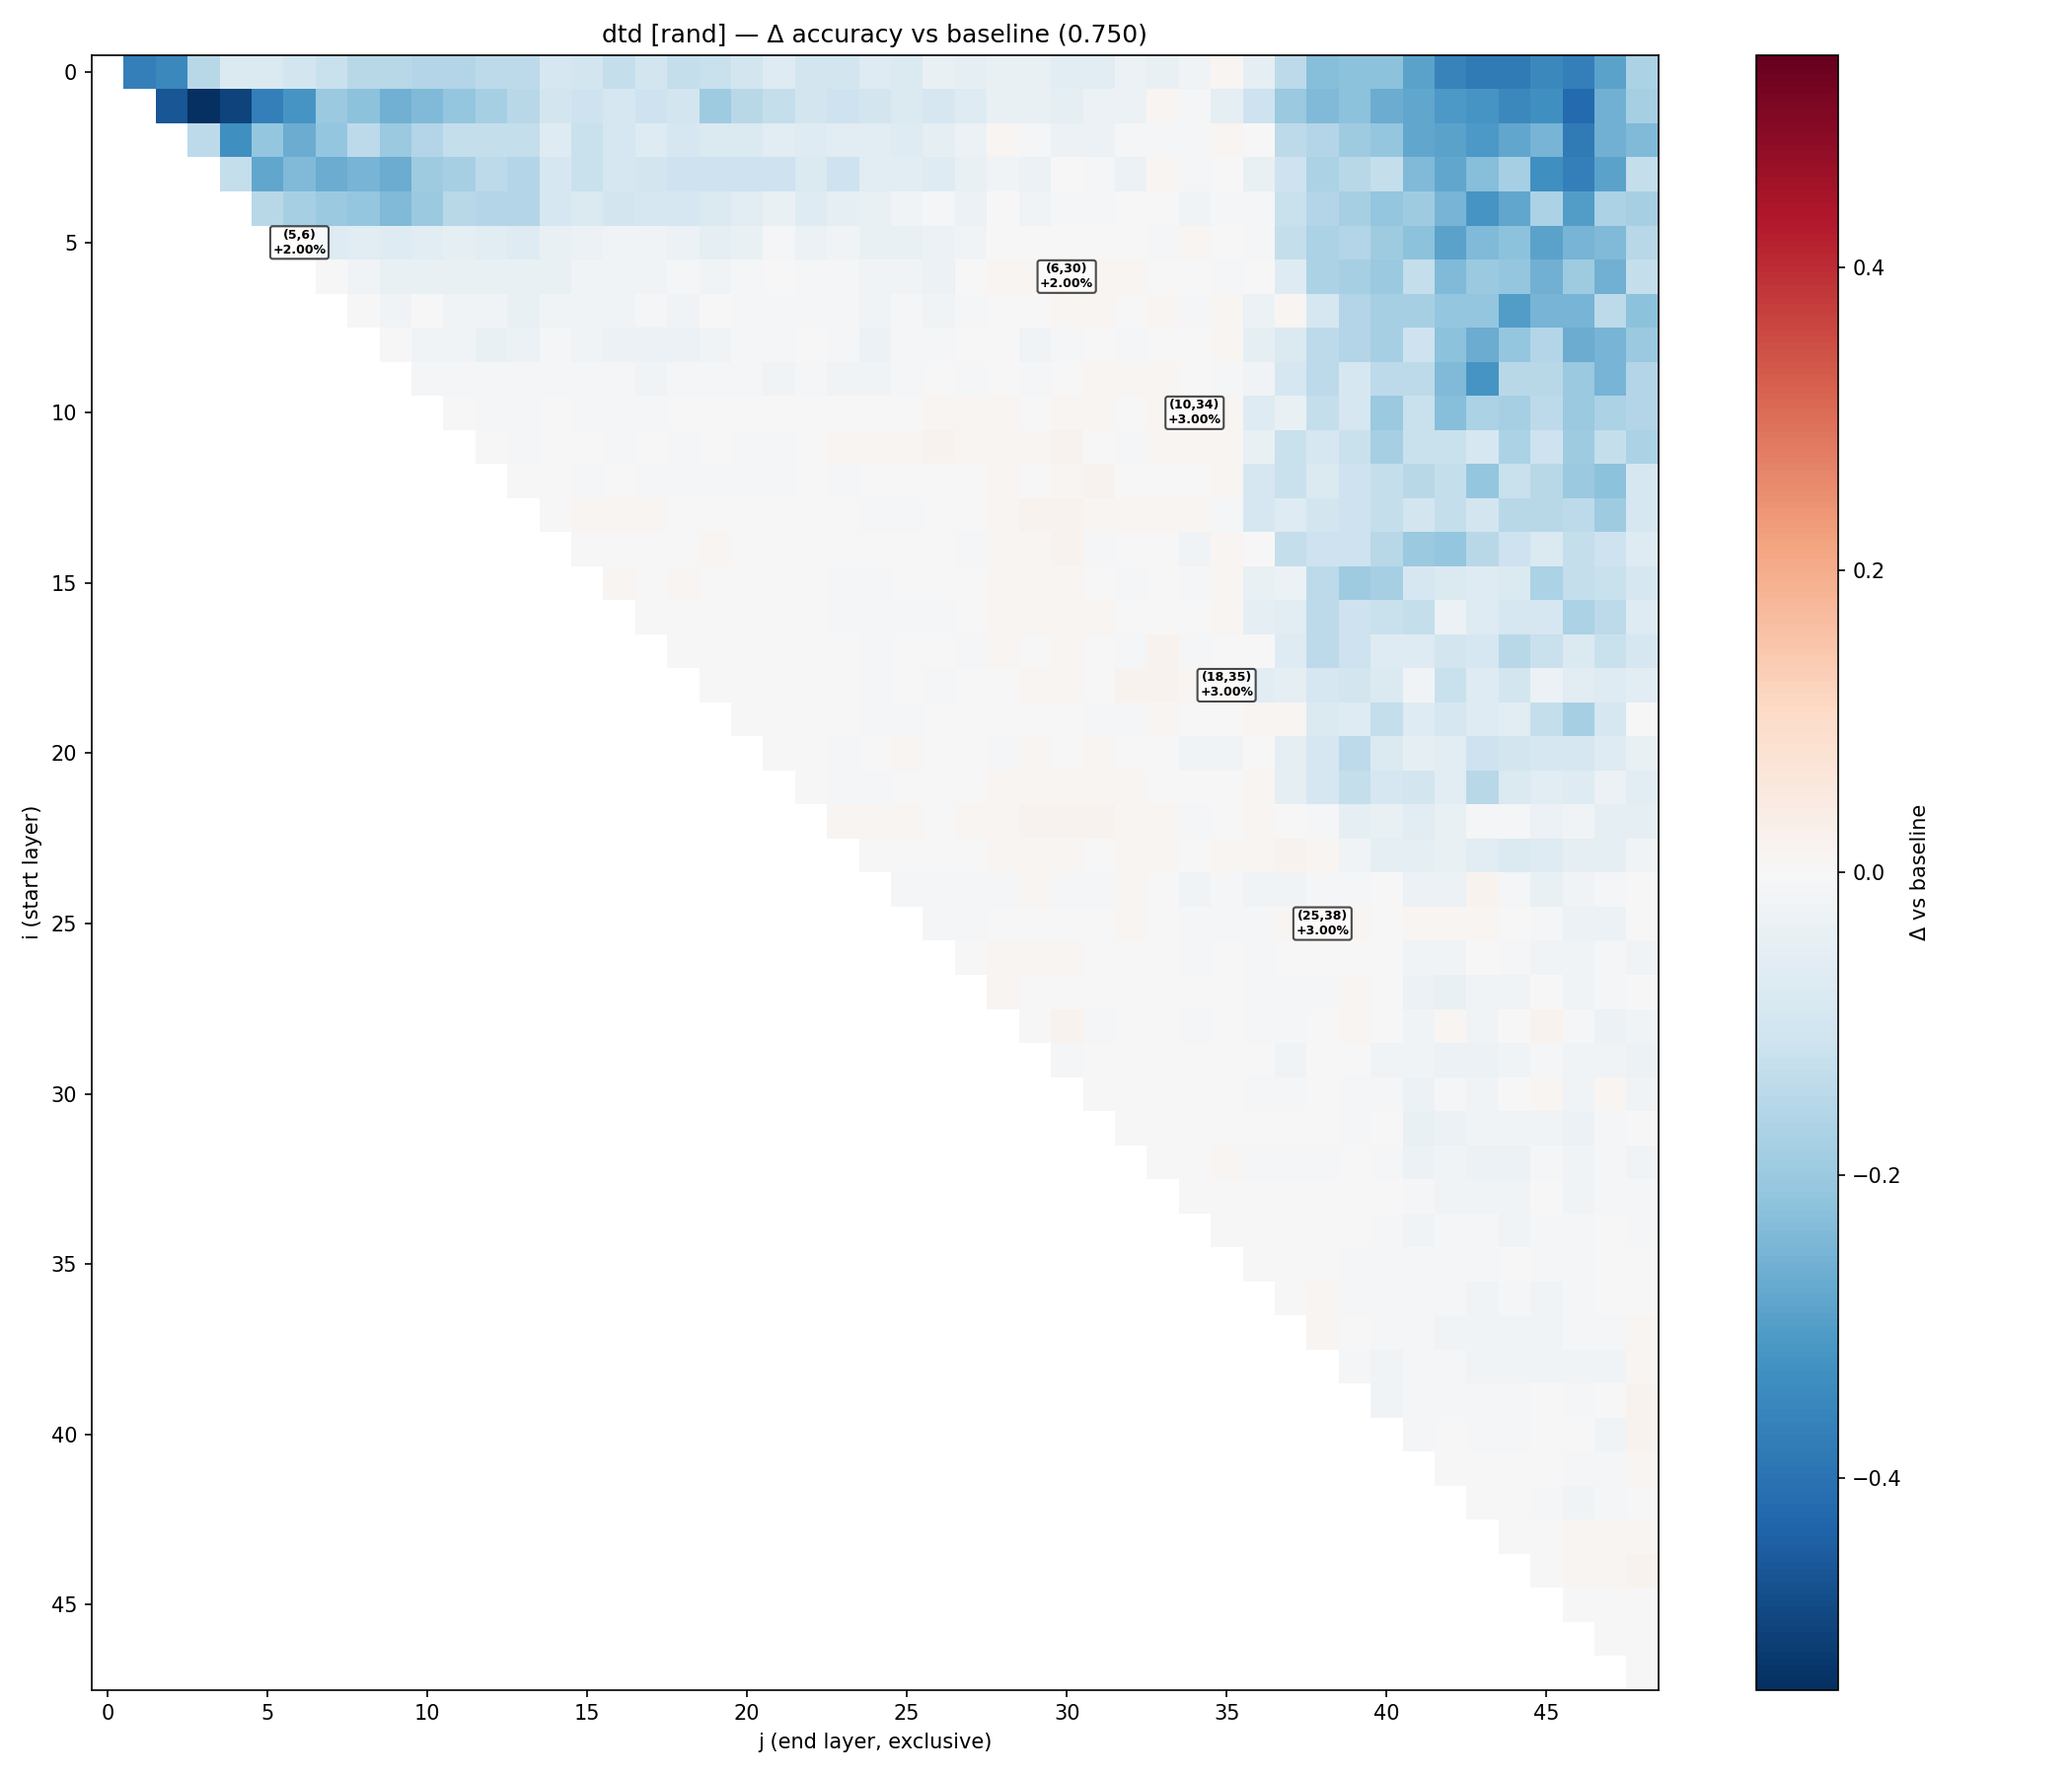
\includegraphics[width=\linewidth]{figures/eva_dtd.png}
\caption{\eva{}, DTD.}
\end{subfigure}%
\begin{subfigure}[t]{0.33\linewidth}
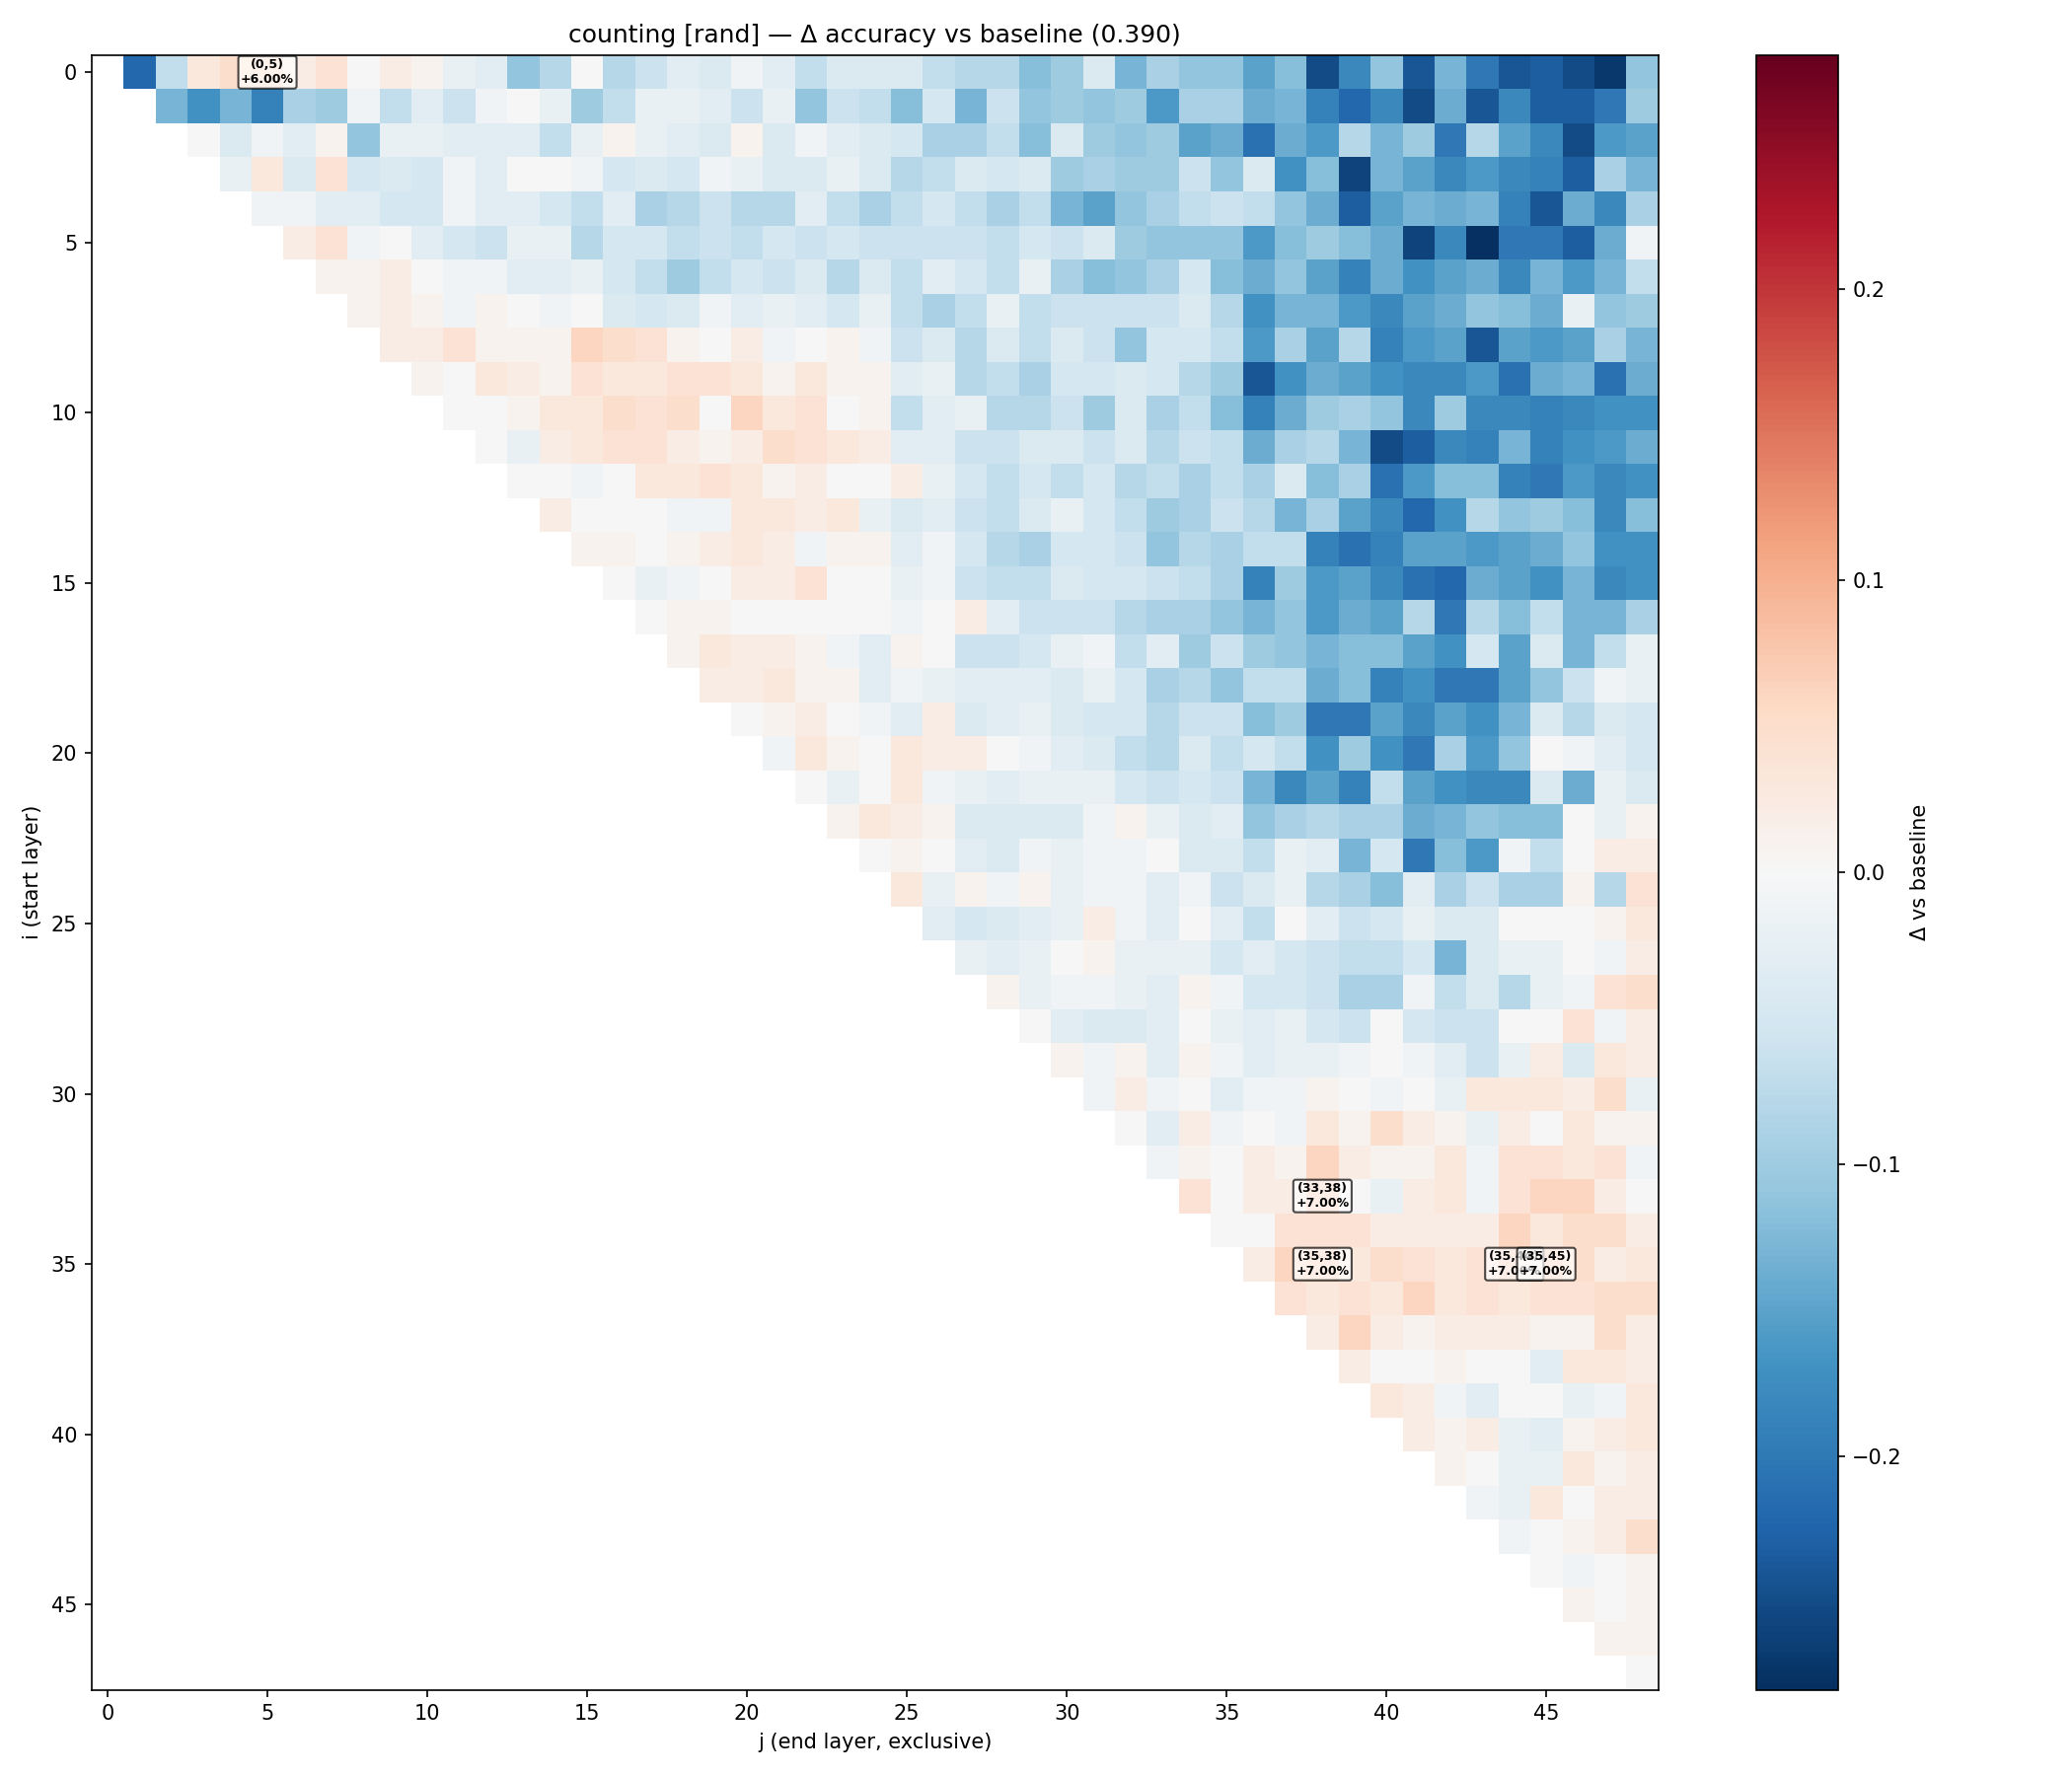
\includegraphics[width=\linewidth]{figures/eva_counting.png}
\caption{\eva{}, counting.}
\end{subfigure}%
\begin{subfigure}[t]{0.33\linewidth}
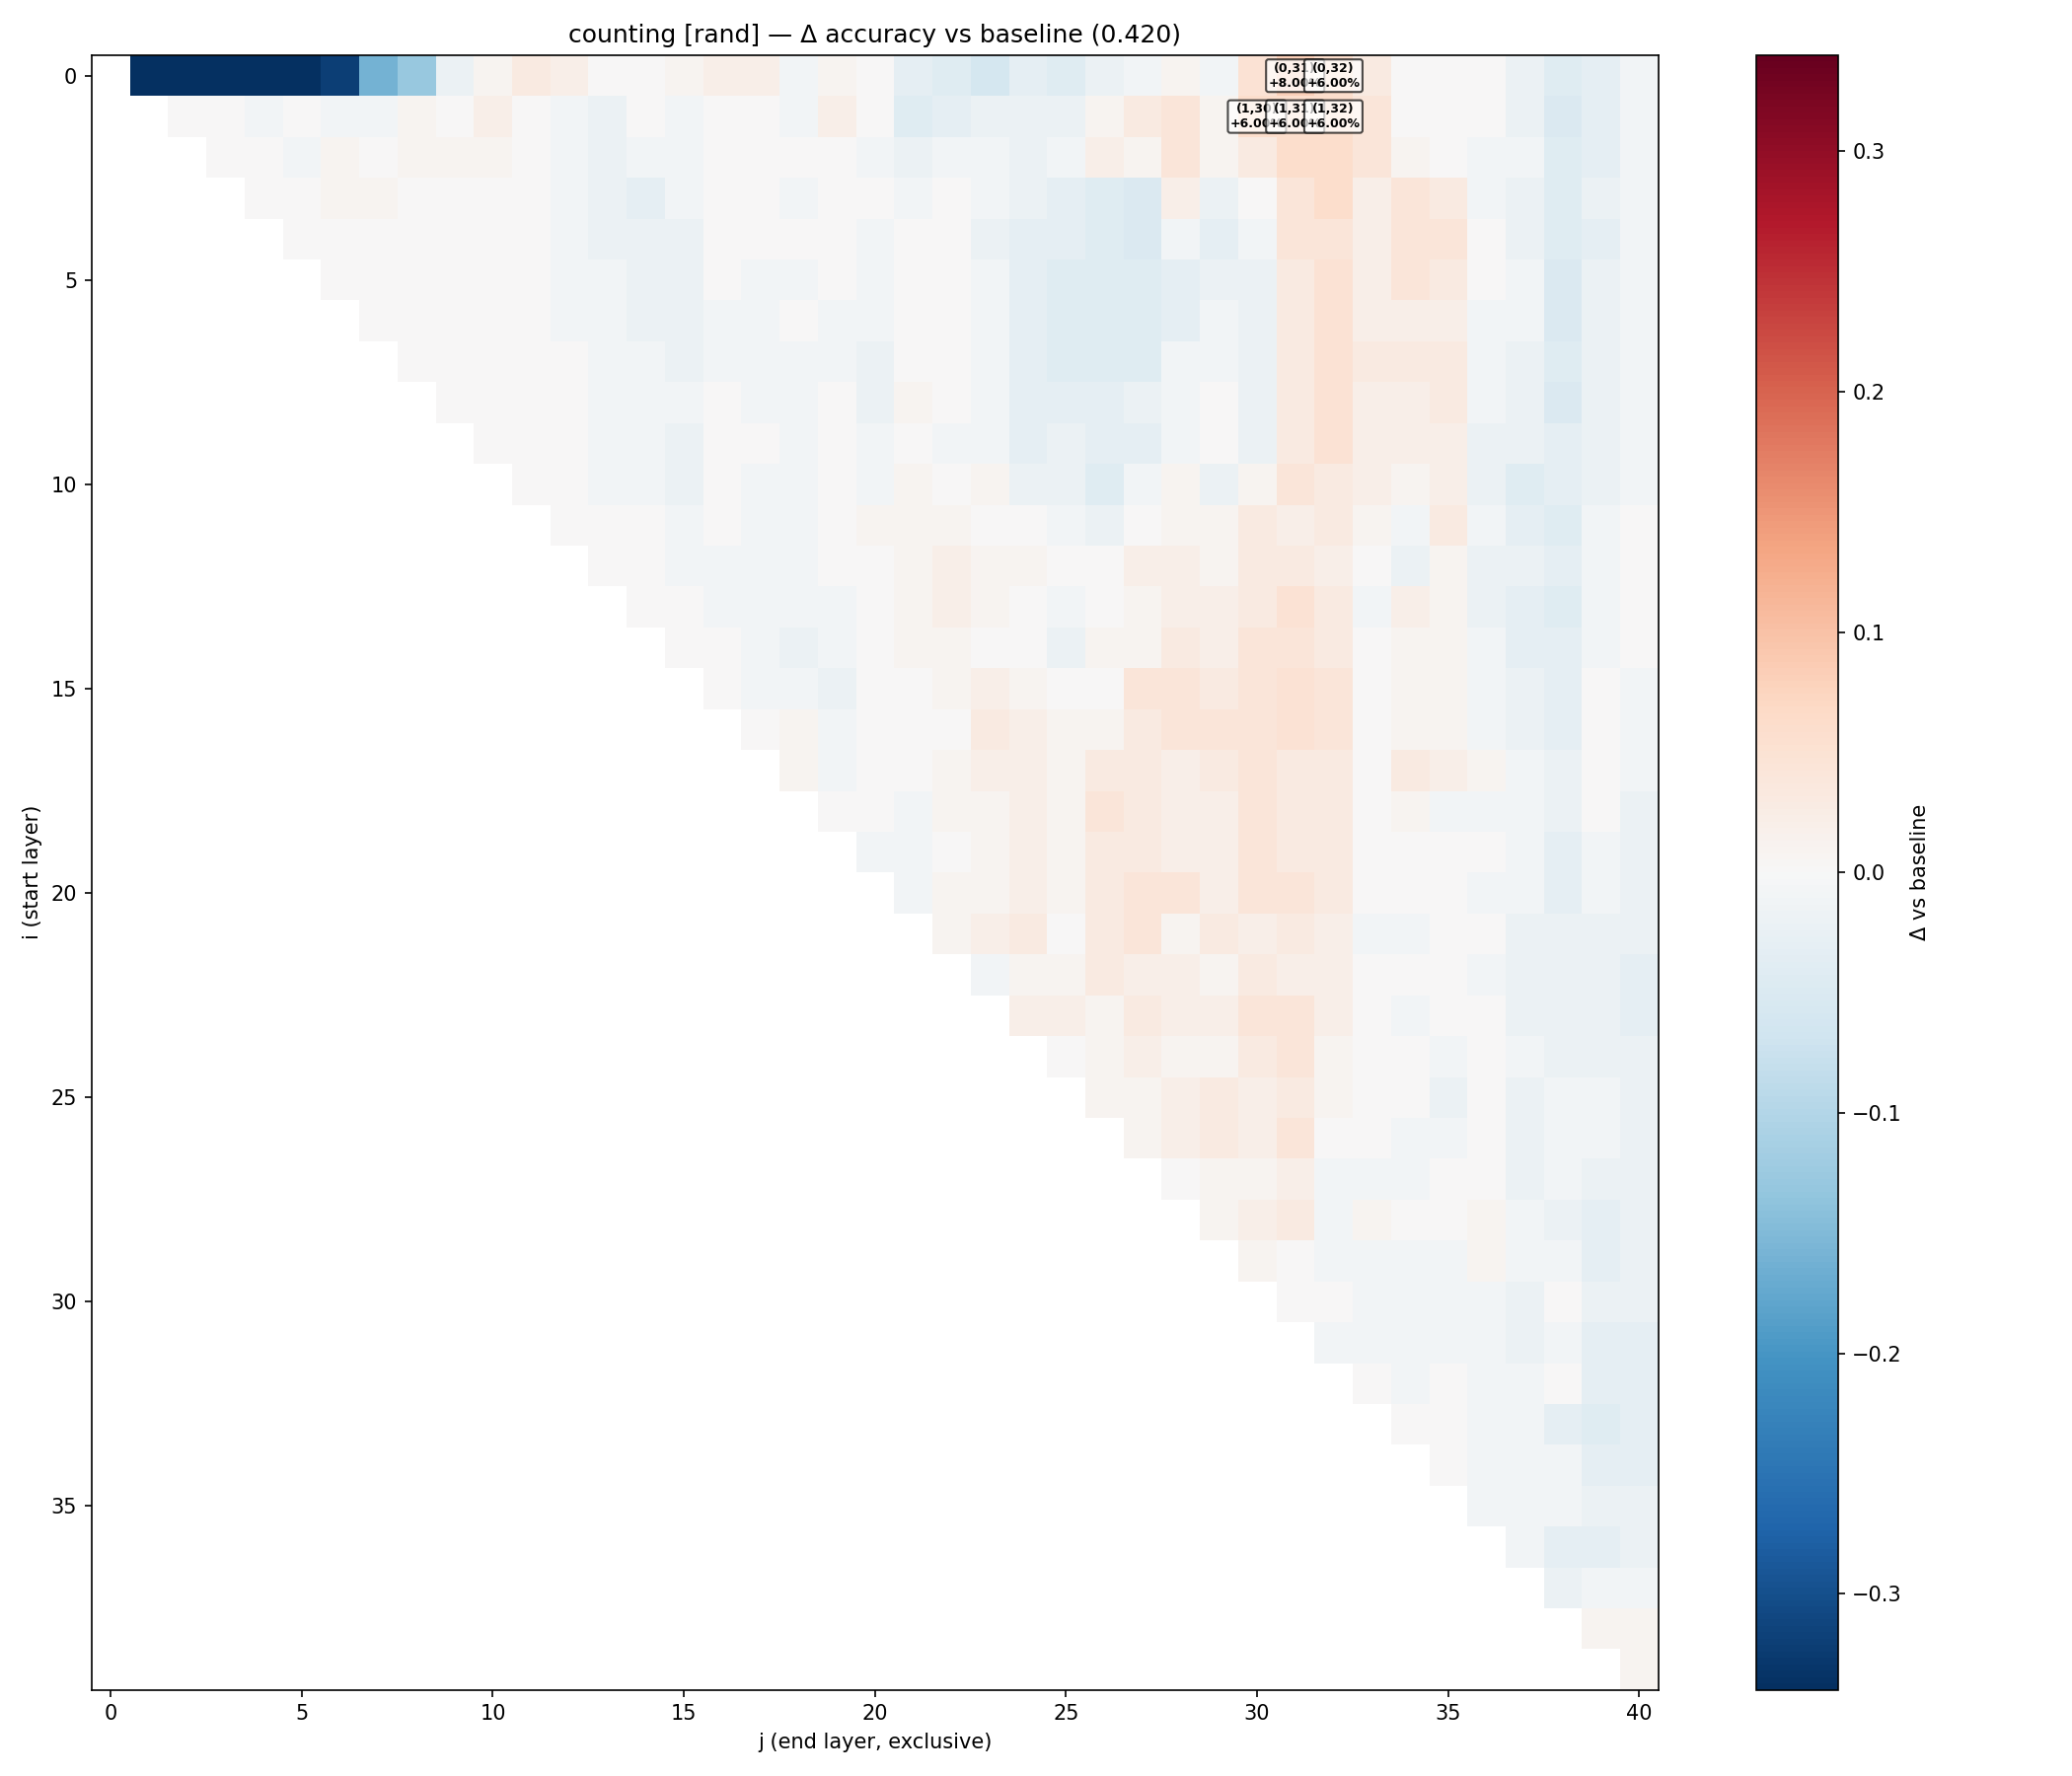
\includegraphics[width=\linewidth]{figures/dino_counting.png}
\caption{\dino{}, counting.}
\end{subfigure}
\caption{\textbf{Representative per-dataset duplication maps} (random
split, $\Delta$accuracy). Texture recognition (a) shows the strongest
early-layer fragility; numerosity (b, c), the probe with the most
headroom, shows the mild positive mid/late-stack structure in both
models.}
\label{fig:perdataset}
\end{figure}

\begin{figure}[h]
\centering
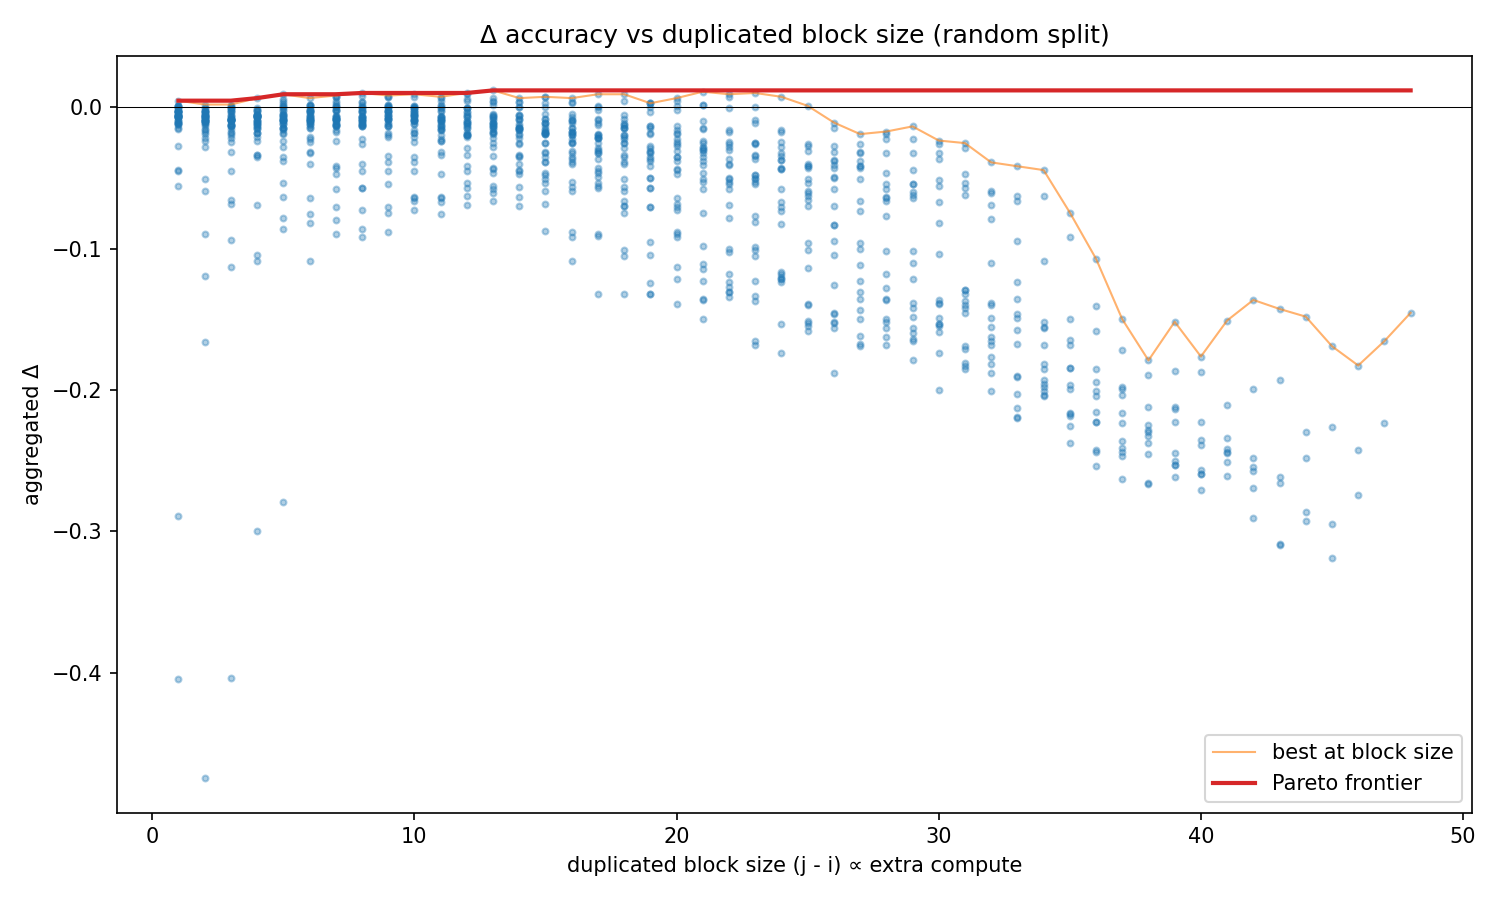
\includegraphics[width=0.6\linewidth]{figures/eva_pareto.png}
\caption{\textbf{Quality/compute Pareto view} (\eva{}, random split):
aggregated $\Delta$accuracy against duplicated block size ($\propto$
extra compute), with the frontier line. No block size offers a favorable
trade at this scale.}
\label{fig:pareto}
\end{figure}

\begin{figure}[h]
\centering
\begin{subfigure}[t]{\linewidth}
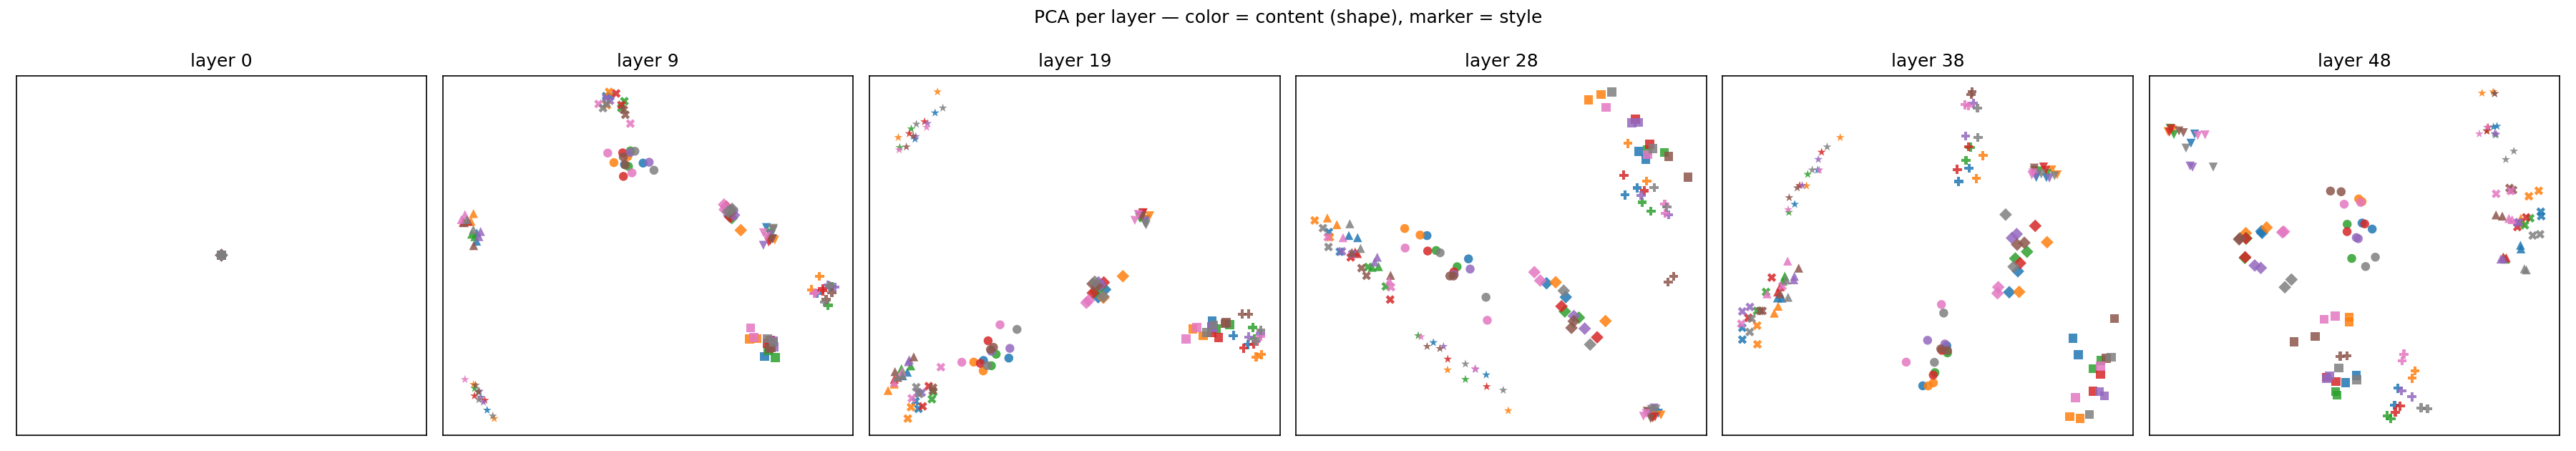
\includegraphics[width=\linewidth]{figures/eva_pca_cls.png}
\caption{\eva{}: cells arrange by style (color mixes within clusters).}
\end{subfigure}
\par\medskip
\begin{subfigure}[t]{\linewidth}
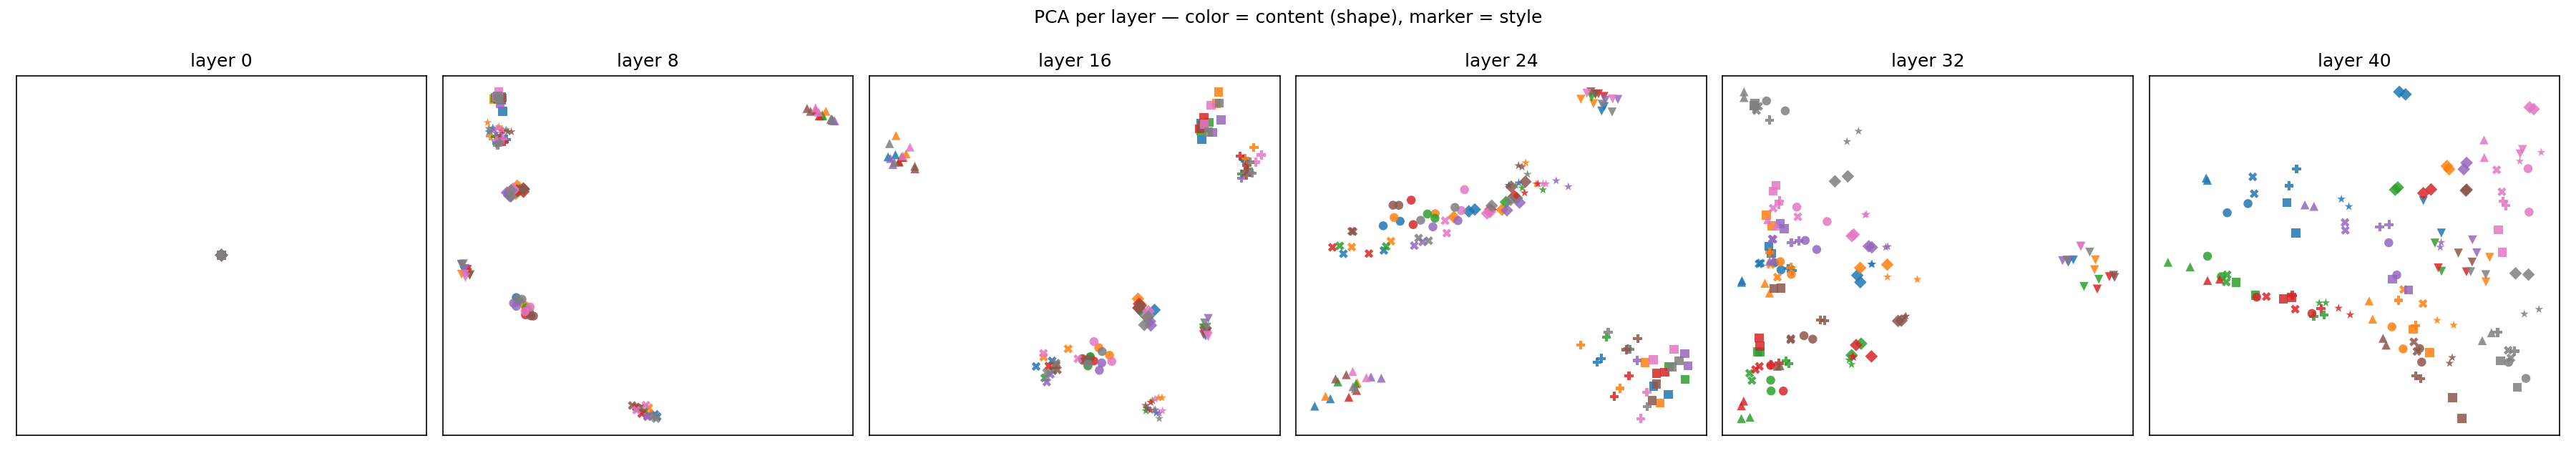
\includegraphics[width=\linewidth]{figures/dino_pca_cls.png}
\caption{\dino{}: late-layer panels cluster by content color.}
\end{subfigure}
\caption{\textbf{Per-layer PCA of anatomy features} (CLS pooling; point
color = shape class, marker = rendering style).}
\label{fig:pca}
\end{figure}

\section{Implementation, verification, and reproducibility}
\label{app:repro}

\textbf{Checkpoint interface facts} (verified against source before any
GPU run): \eva{} ships no preprocessor configuration (its model card uses
the OpenAI CLIP processor, which we adopt); its encoder blocks take two
required positional mask arguments; its vision tower applies a
post-layer-norm before pooling, which we include in the probed feature.
\dino{} computes rotary position embeddings once per input, shared by all
blocks; its four register tokens~\citep{darcet2024vision} are excluded
from patch pooling; its final norm is included in the probed feature. For
both models, our re-implemented forward path reproduces the checkpoint's
own \texttt{forward} to numerical identity on random-initialization
tests, and cached-path/direct-path equality is asserted on the real
checkpoints before scanning.

\textbf{Verification.} A CPU-only test suite (25 tests) covers the
scanner algebra (cache/direct equivalence, repetition semantics,
validation), probe scoring, borderline stratification, every synthetic
confound control (non-overlap, area matching, half-marginal identity,
boundary margins, label validity), anatomy pair-category combinatorics,
recovery of planted structure, and an end-to-end miniature pipeline
(scan $\to$ resume $\to$ figures $\to$ report $\to$ confirmation) with a
dummy transformer. A simulated mid-scan crash repairs bit-identically
under resume.

\textbf{Determinism.} All sampling is seeded (reference/candidate
selection, split draws, confirmation images and references, control
configurations, synthetic generation, class subsets); models run in
evaluation mode in fp16. Residual GPU nondeterminism is below the
quantization of 100-image accuracies.

\textbf{Software.} PyTorch 2.13 (CUDA); \texttt{transformers} 4.49 for
the \eva{} arm (its remote code predates API changes in 4.50+) and 5.14
for the \dino{} arm, in separate environments; \texttt{datasets} 2.21
($<3$, required by the script-based ImageNet loader). Complete pins,
seeds, and the full decision log accompany the repository.

\textbf{Scale of the experiment.} 21{,}956 configuration--dataset
evaluations (sweeps), 1{,}936 single-layer repetition evaluations, 880
confirmation evaluations (40 configurations $\times$ 11 datasets $\times$
2 stages of features), and two anatomy passes, in $\approx 33.5$ GPU-hours
on one H100.

\end{document}
